\documentclass[12pt]{article}
\usepackage{fontspec}
\usepackage{graphicx}
\usepackage{geometry}
\usepackage{float}
\usepackage{hyperref}
\usepackage{tikz}
\usepackage{polyglossia}
\setmainlanguage{farsi}
\setotherlanguage{english}
\newfontfamily\englishfont{Times New Roman}
\newfontfamily\persianfont[Script=Arabic]{XB Zar.ttf}




\geometry{a4paper, margin=2.5cm}
\usepackage{setspace}
\onehalfspacing
\usepackage{titling}
\usepackage{etoolbox}
\usepackage[backend=biber,style=numeric,sorting=none]{biblatex}
%%%%%%%%%%%%%%%%%%%%%%%%%%%%%%%%%%%%%%%%%%%%%%%%%%%%%%%%%%%%%%%%%%%%%%%%%%%%%
\makeatletter
\newcommand{\persiandigit}[1]{%
	\ifcase#1 ۰\or ۱\or ۲\or ۳\or ۴\or ۵\or ۶\or ۷\or ۸\or ۹\fi
}
\DeclareFieldFormat{labelnumber}{\persiandigit{#1}}
\makeatother
%%%%%%%%%%%%%%%%%%%%%%%%%%%%%%%%%
\newcommand{\persianordinal}[1]{%
	\ifcase#1
	\or اول%
	\or دوم%
	\or سوم%
	\or چهارم%
	\or پنجم%
	\or ششم%
	\or هفتم%
	\or هشتم%
	\or نهم%
	\or دهم%
	\or یازدهم%
	\or دوازدهم%
	\or سیزدهم%
	\or چهاردهم%
	\or پانزدهم%
	\or شانزدهم%
	\or هفدهم%
	\or هجدهم%
	\or نوزدهم%
	\or بیستم%
	\else #1\fi
}

\newcommand{\persianordinalpage}{\persianfont\persianordinal{\value{page}}}


%%%%%%%%%%%%%%%%%%%%%%%%%%%%%%%%%%%%%%%%%%%%%%%%%%%%%%%%%%%%%%%%%%%%%%%%%%%%%
\begin{filecontents}{\jobname.bib}
@online{man7-getpgrp,
    author    = {{Michael Kerrisk}},
    title     = {getpgrp(2) - Linux manual page},
    year      = {2024},
    url       = {https://man7.org/linux/man-pages/man2/getpgrp.2.html},
    note      = {Accessed: 2025-08-02}
}

@online{man7-setpgid,
    author    = {{Michael Kerrisk}},
    title     = {setpgrp(2) - Linux manual page},
    year      = {2024},
    url       = {https://man7.org/linux/man-pages/man2/setpgid.2.html},
    note      = {Accessed: 2025-08-02}
}

@online{man7-credentials,
    author    = {{Michael Kerrisk}},
    title     = {credentials(7) – Process Group and Session Model},
    year      = {2024},
    url       = {https://man7.org/linux/man-pages/man7/credentials.7.html},
    note      = {Accessed: 2025-08-02}
}

@online{wikipedia-zombie-process,
    author    = {{Wikipedia contributors}},
    title     = {Zombie process},
    year      = {2025},
    url       = {https://en.wikipedia.org/wiki/Zombie_process},
    note      = {Accessed: 2025-08-02}
}

\end{filecontents}

\addbibresource{\jobname.bib}

\defbibheading{bibliography}[]{%
	\begin{RTL}
		\section*{مراجع}
	\end{RTL}
}

%%%%%%%%%%%%%%%%%%%%%%%%%%%%%%%%%%%%%%%%%%%%%%%%%%%%%%%%%%%%%%%%%%%%%%%%%%%%%

\begin{document}
	
	% ==============================
	% Title Page
	% ==============================
	\begin{titlepage}
		\centering
		\vspace*{1cm}
		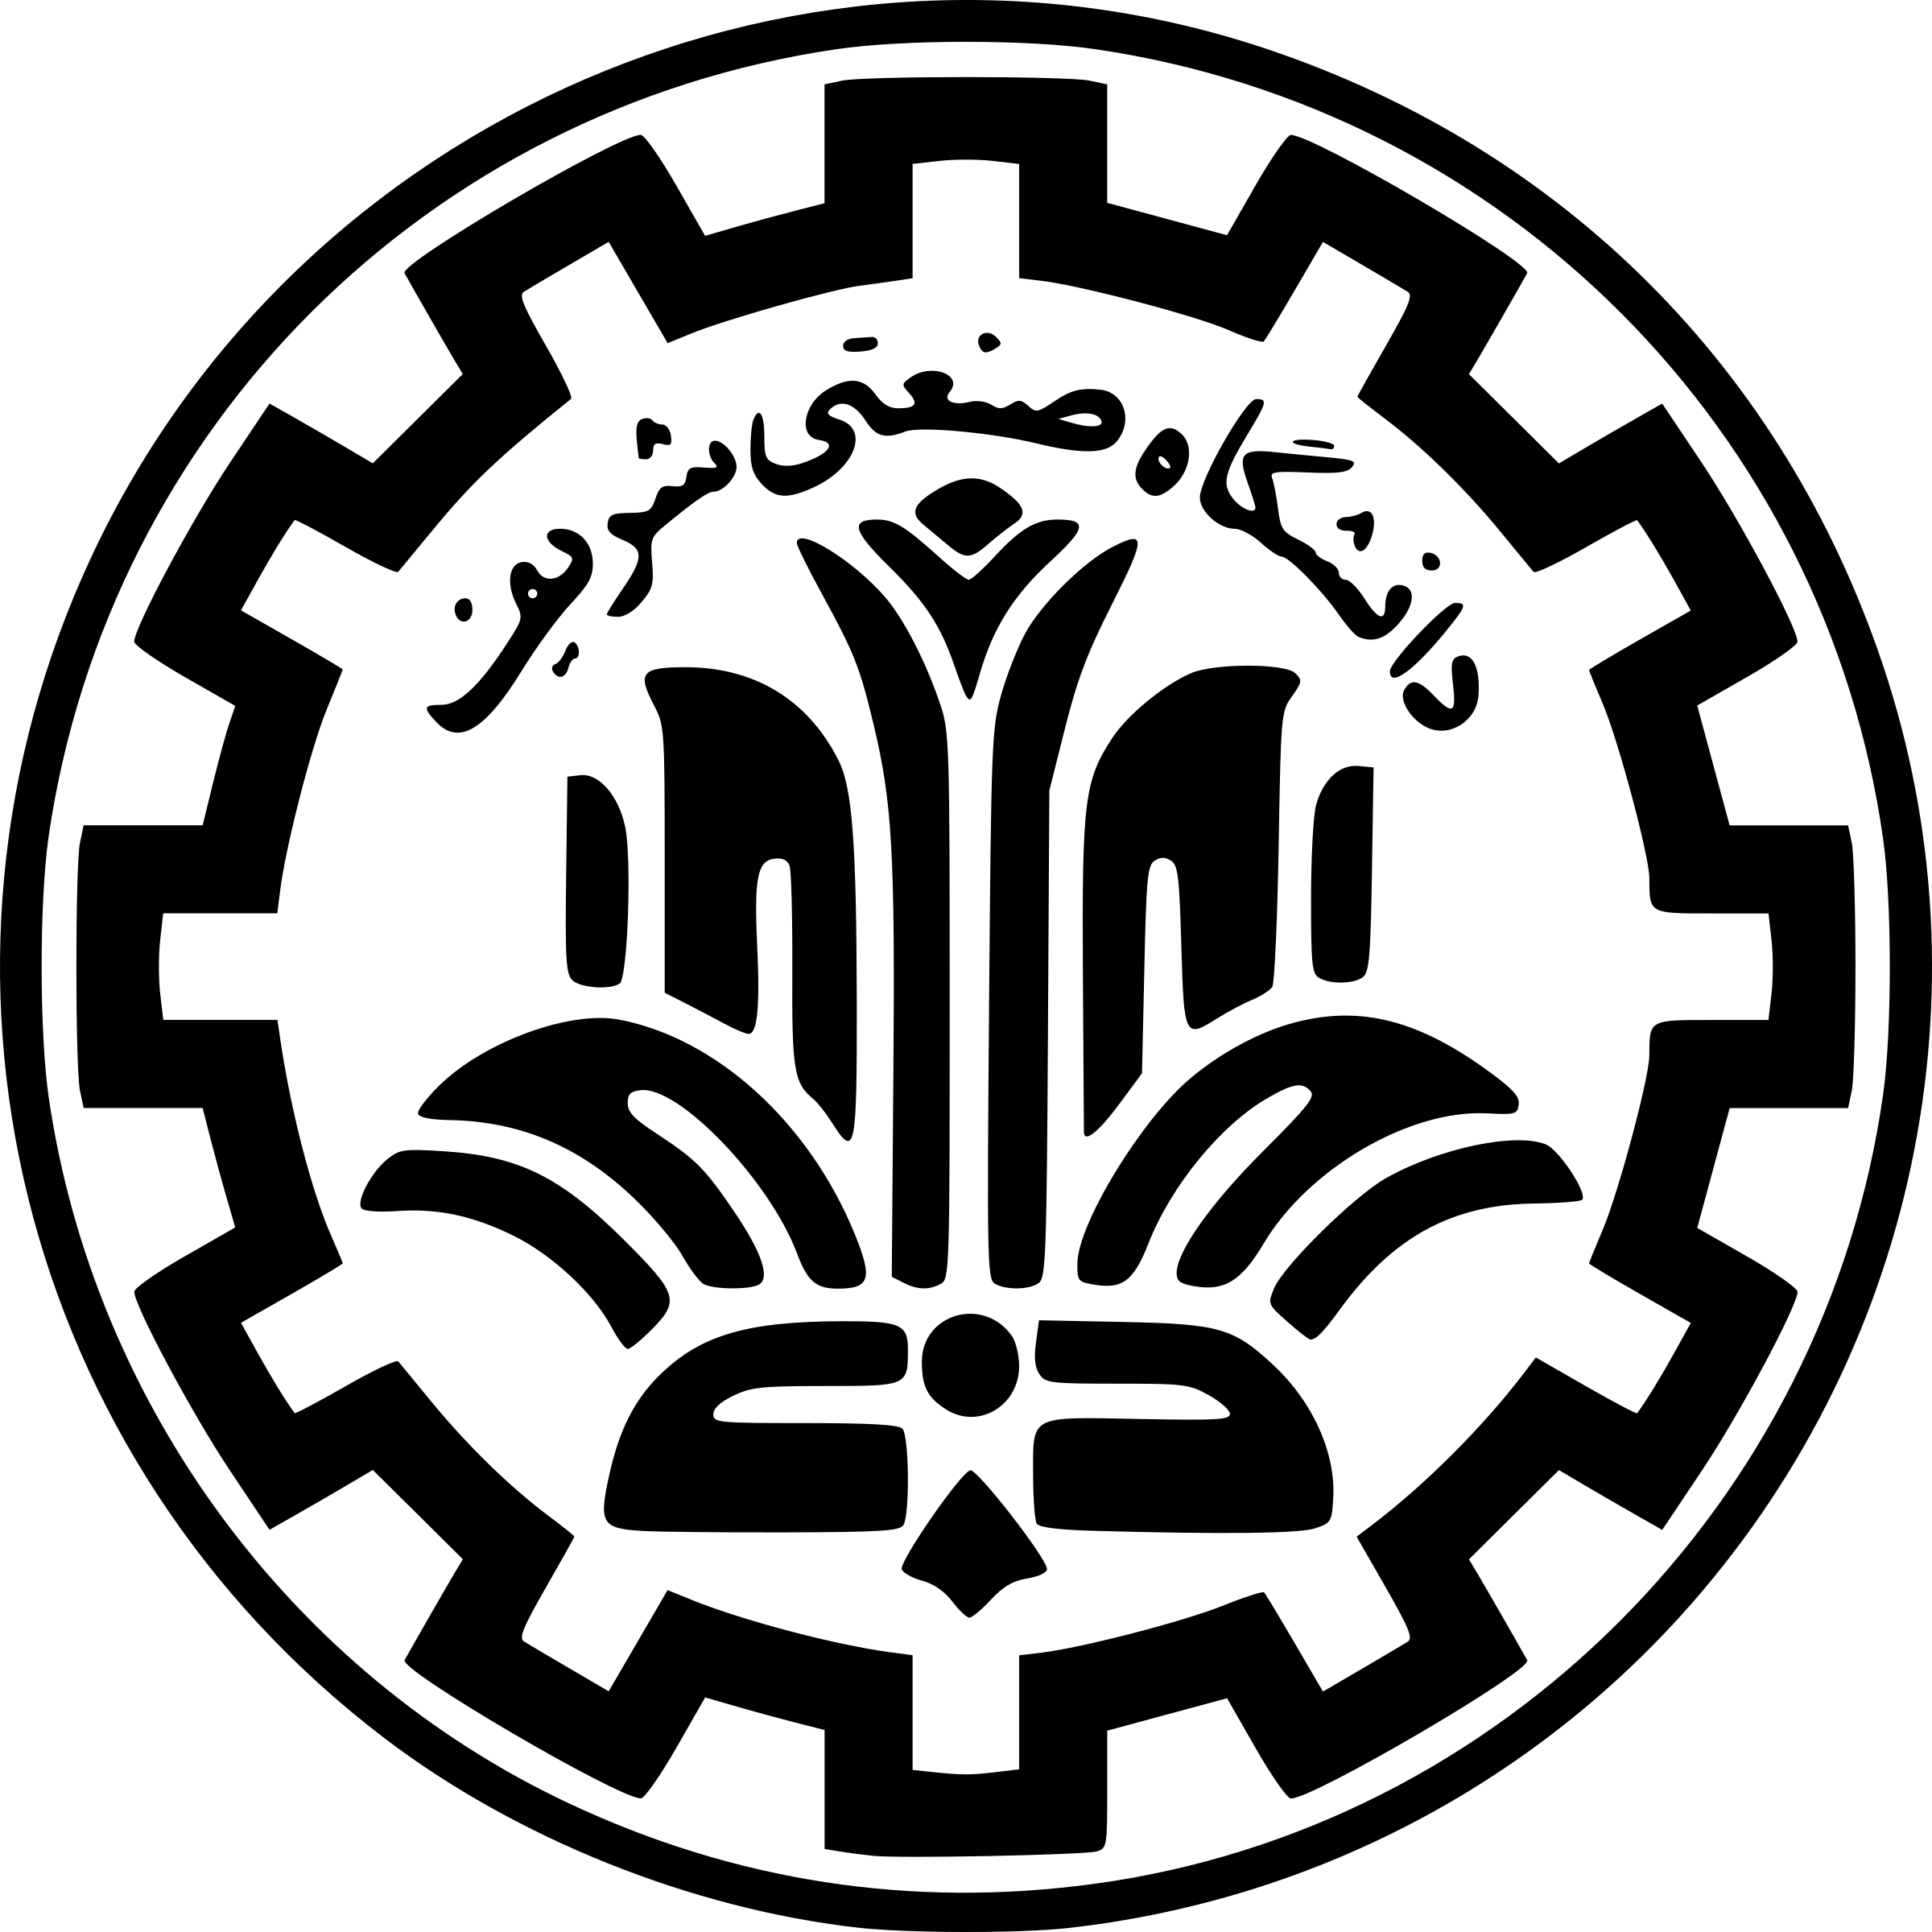
\includegraphics[width=4cm]{sharif.png}\\[1.5cm]
		{\Large\textbf{دانشگاه صنعتی شریف}}\\[0.5cm]
		{\large\textbf{دانشکده‌ی مهندسی کامپیوتر}}\\[1.5cm]
		{\Huge\textbf{گزارش کار آزمایشگاه}}\\[0.5cm]
		{\LARGE\textbf{آزمایشگاه سیستم‌های عامل}}\\[2cm]
		
		\textbf{گزارش آزمایش شماره ۴}\\
		(ایجاد و اجرای پردازه‌ها)
		
		\vfill
		\begin{tabular}{rl}
			\textbf{شماره‌ی گروه:} & ۲۰ \\
			\textbf{گروه:} &
			ارشیا یوسف‌نیا (۴۰۱۱۱۰۴۱۵) \\
			& محمدعارف زارع زاده (۴۰۱۱۰۶۰۱۷) \\
			\textbf{استاد درس:} & دکتر بیگی \\
			\textbf{تاریخ:} & تابستان ۱۴۰۴ \\
		\end{tabular}
	\end{titlepage}
	
	% ==============================
	% Persian Ordinal Page Numbering
	% ==============================
	\clearpage
	\setcounter{page}{1}
	\renewcommand{\thepage}{\persianordinalpage}
	
	\tableofcontents
	\clearpage
	\listoffigures
	\clearpage
	\listoftables
	
	% ==============================
	% Switch to Persian Digits (۱, ۲, ۳, ...)
	% ==============================
	\clearpage
	\setcounter{page}{1}
	\pagenumbering{arabic}
	\renewcommand{\thepage}{\persianfont\arabic{page}}
	
	
	% ==============================
	% Main Content
	% ==============================
        \section{شرح آزمایش}
        \subsection{مشاهده‌ی پردازه‌های سیستم و \textenglish{PID} آنها}

        \begin{enumerate}
        \item 
        با دستور
        \textenglish{ps aux}
        می‌توان لیست تمام پردازه‌های درحال اجرا در سیستم را مشاهده کرد.

        \begin{figure}[H]
		\centering
		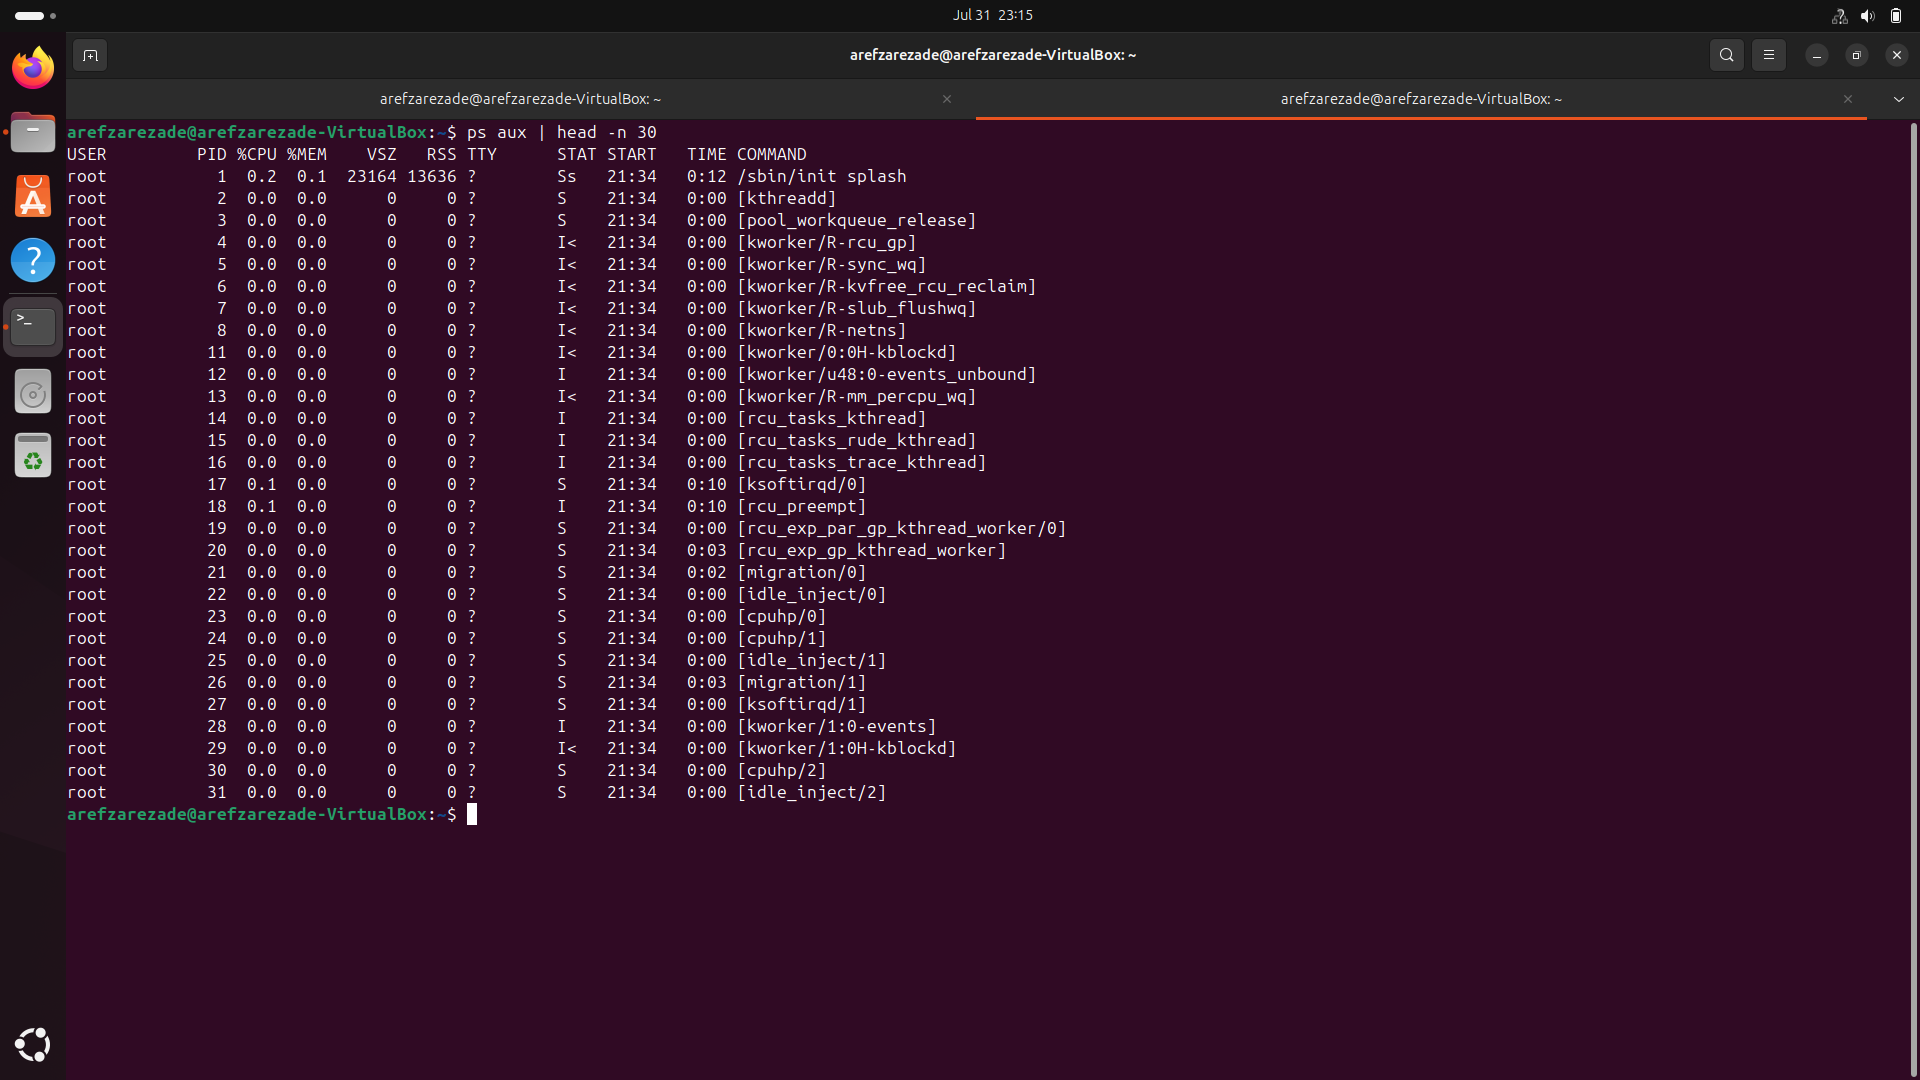
\includegraphics[width=0.8\textwidth]{report4-resources/1.png}
		\caption{سی پردازه‌ی اول درحال اجرا در سیستم}
            \label{im1}
	\end{figure}

        \item 

        همانطور که در شکل 
        \ref{im1}
        می‌توان مشاهده کرد، پردازه‌ای که دارای
        \textenglish{PID=1}
        ‌می‌باشد، 
        \textenglish{init}
        نام دارد. در شکل 
        \ref{im2}
        می‌توان اطلاعات مربوط به
        \textenglish{man init}
        را مشاهده کرد. در ادامه، توضیحاتی درمورد آن می‌دهیم.

        \begin{figure}[H]
		\centering
		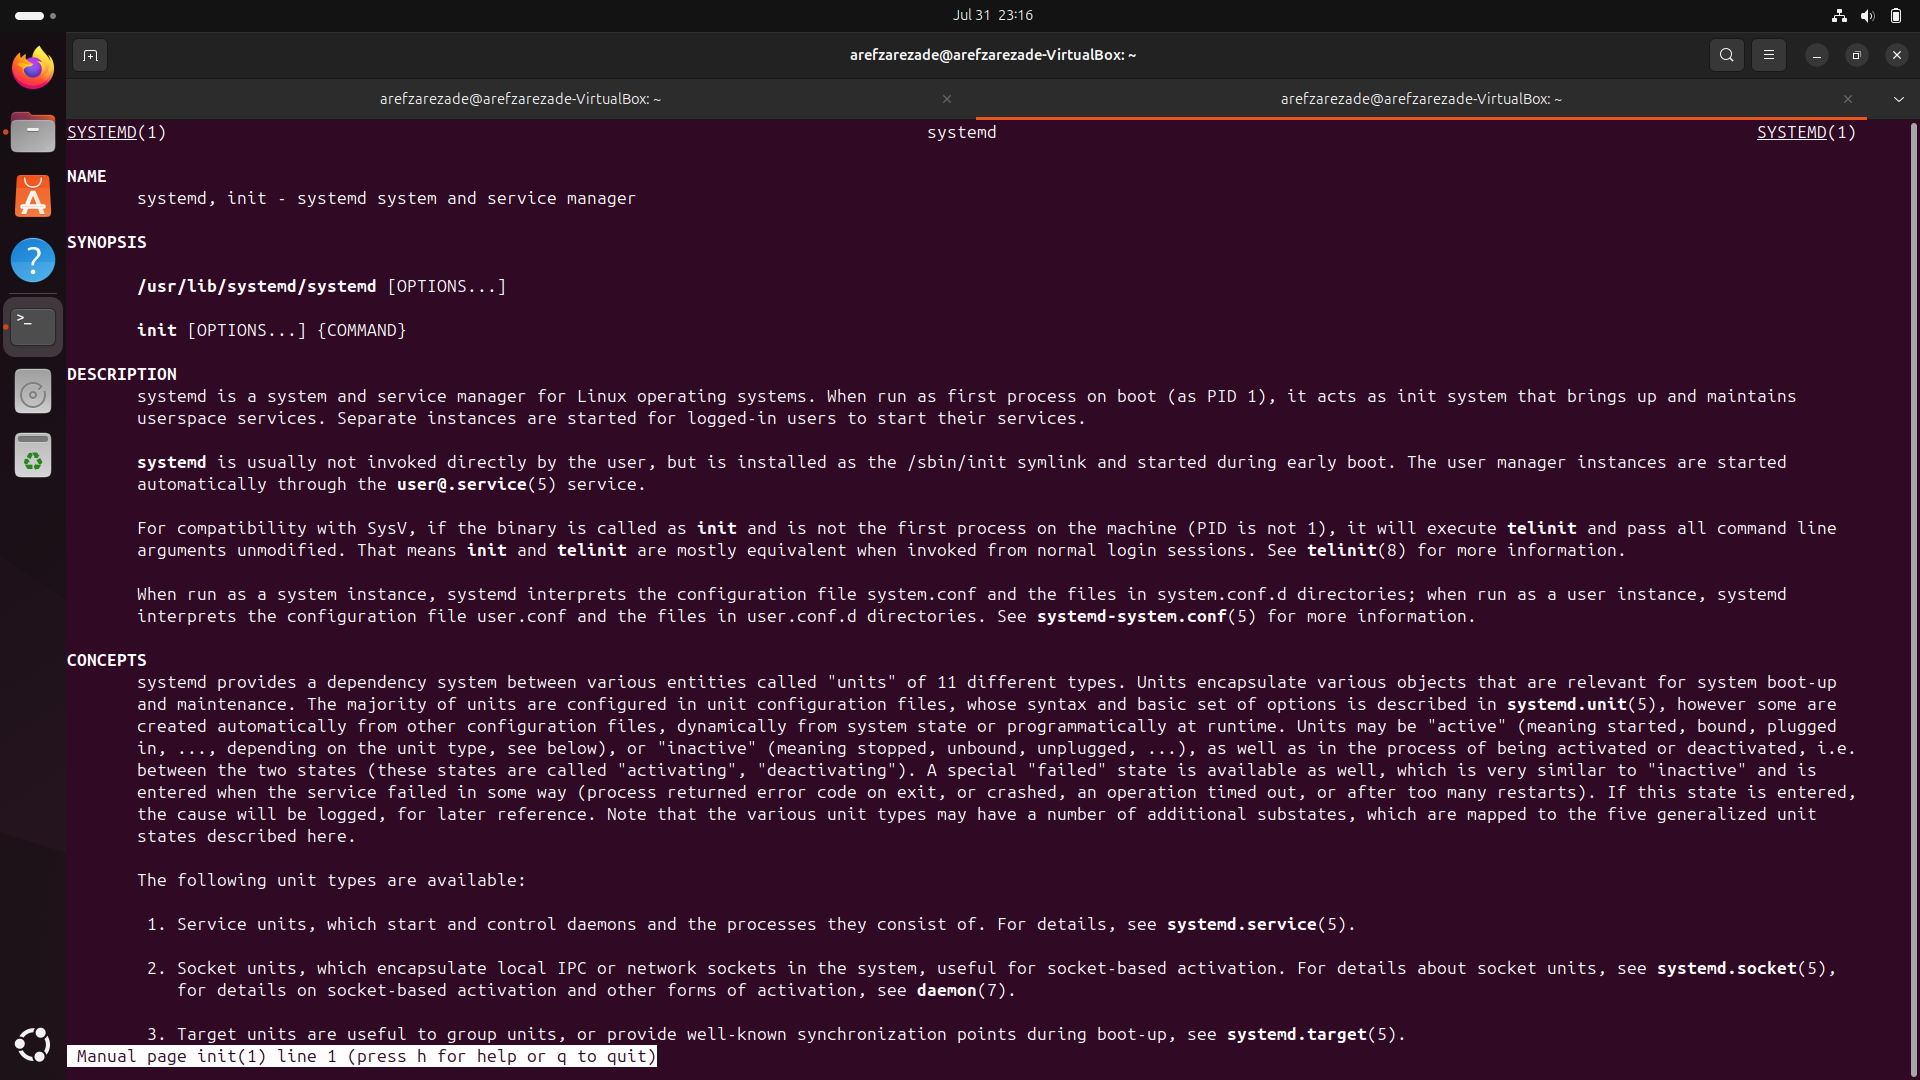
\includegraphics[width=0.8\textwidth]{report4-resources/2.png}
		\caption{توضیحات دستور \textenglish{man} درباره‌ی پردازه‌ی \textenglish{init}}
            \label{im2}
	\end{figure}

        هنگام روشن کردن سیستم،
        \textenglish{bootloader}
        ابتدا هسته را لود کرده و هسته بعد از کارهایی مانند آماده کردن حافظه، 
        \textenglish{file system}
        و ...
        پردازه‌ی 
        \textenglish{init}
        را اجرا می‌کند. این پردازه، با خواندن فایل‌های مربوط به
        \textenglish{configuration}
        سیستم را به درستی آماده کرده و سرویس‌ها و پردازه‌هایی که برای سیستم مورد نیاز هستند را اجرا می‌کند. به بیان دیگر، این پردازه پدر تمام پردازه‌های سیستم است و مدیریت پردازه‌ها برعهده‌ی آن است.

        \item 
        تابع
        \textenglish{getpid()}
        تابعی است که 
        \textenglish{PID}
        مربوط به پردازه‌ای که آن را فراخوانده است را خروجی می‌دهد. خروجی آن از نوع
        \textenglish{pid\_t}
        است که در اکثر مواقع مانند 
        \textenglish{int}
        عمل می‌کند. در شکل
        \ref{im3}
        می‌توانید کدی که از آن استفاده می‌کند و اجرا شدن آن را مشاهده کنید.

        \begin{figure}[H]
		\centering
		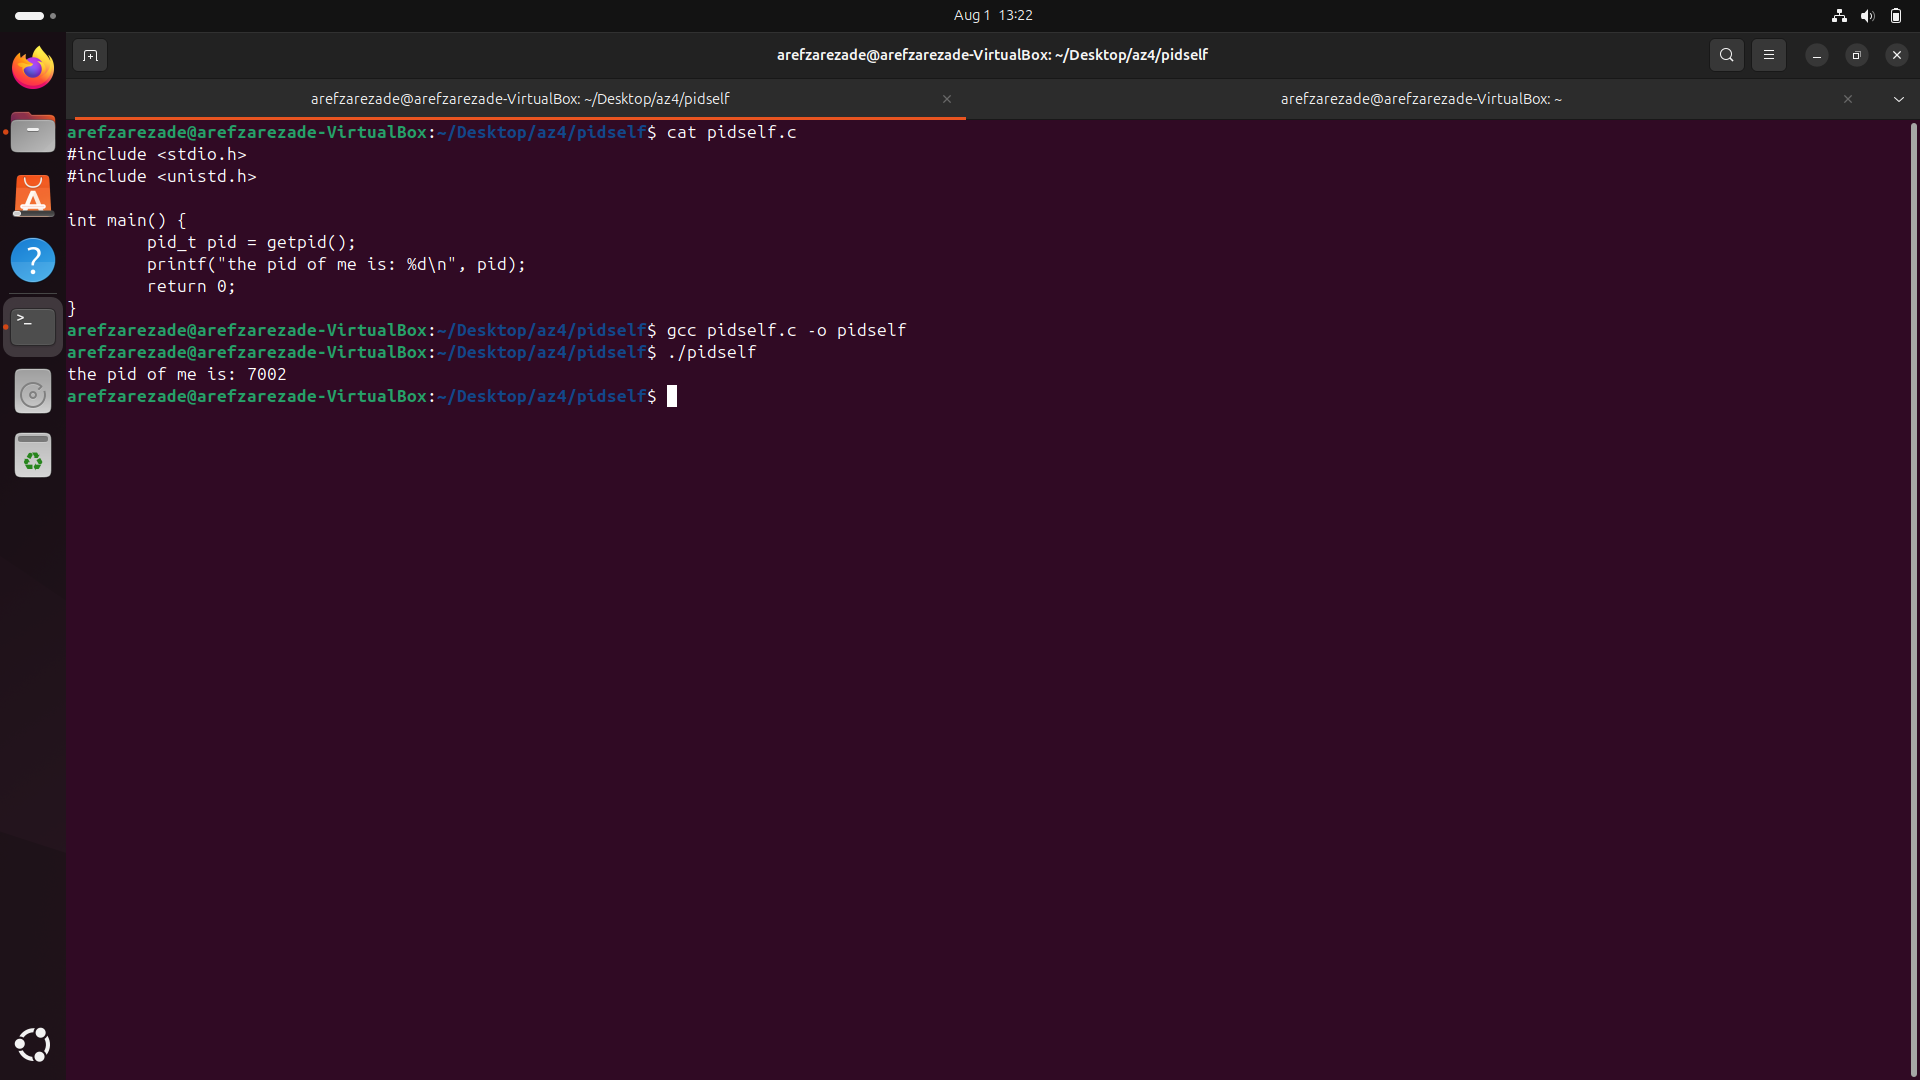
\includegraphics[width=0.8\textwidth]{report4-resources/3.png}
		\caption{چاپ \textenglish{PID} با کمک دستور \textenglish{getpid()}}
            \label{im3}
	\end{figure}
        \end{enumerate}

        \subsection{ایجاد یک پردازه‌ی جدید}

        \begin{enumerate}
        \item 
        در شکل 
        \ref{im4}
        می‌توانید کد این برنامه و خروجی آن و همچنین پردازه‌ی پدر آن را مشاهده کنید.

        \begin{figure}[H]
		\centering
		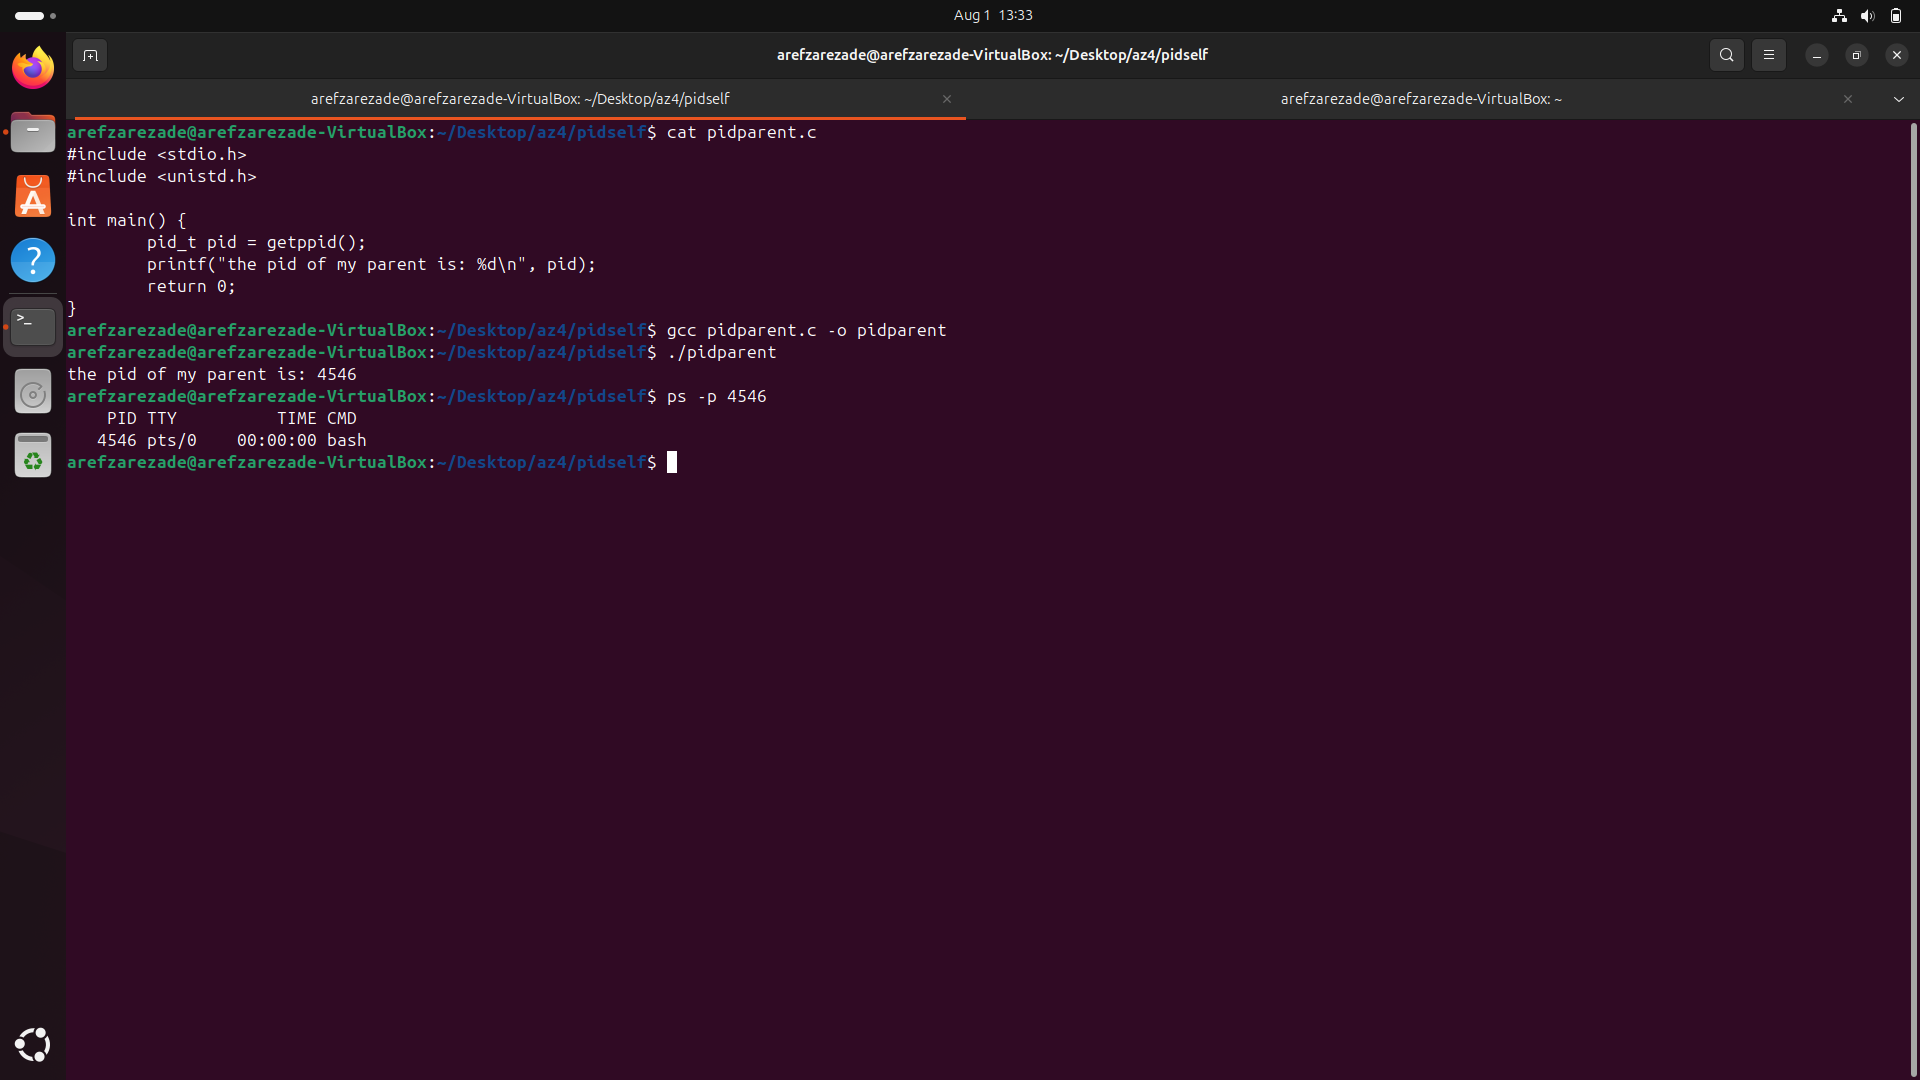
\includegraphics[width=0.8\textwidth]{report4-resources/4.png}
		\caption{مشاهده‌ی پردازه‌ی پدر با \textenglish{getppid()}}
            \label{im4}
	\end{figure}

        همانطور که می‌توان مشاهده کرد، پردازه‌ی پدر این برنامه 
        \textenglish{bash}
        است. وقتی که ترمینال را اجرا می‌کنیم، ترمینال یک پردازه‌ی
        \textenglish{bash}
        را ایجاد می‌کند که وظیفه‌اش اجرای دستورات وارد شده در ترمینال است. وثتی برنامه‌ای را در ترمینال اجرا می‌کنیم، این پردازه‌ی
        \textenglish{bash}
        یک پردازه‌ی جدید ساخته که آن پردازه برنامه را اجرا می‌کند.

        \item 
        در شکل 
        \ref{im5}
        می‌توانید این کد و اجرای آن را مشاهده کنید.

        \begin{figure}[H]
		\centering
		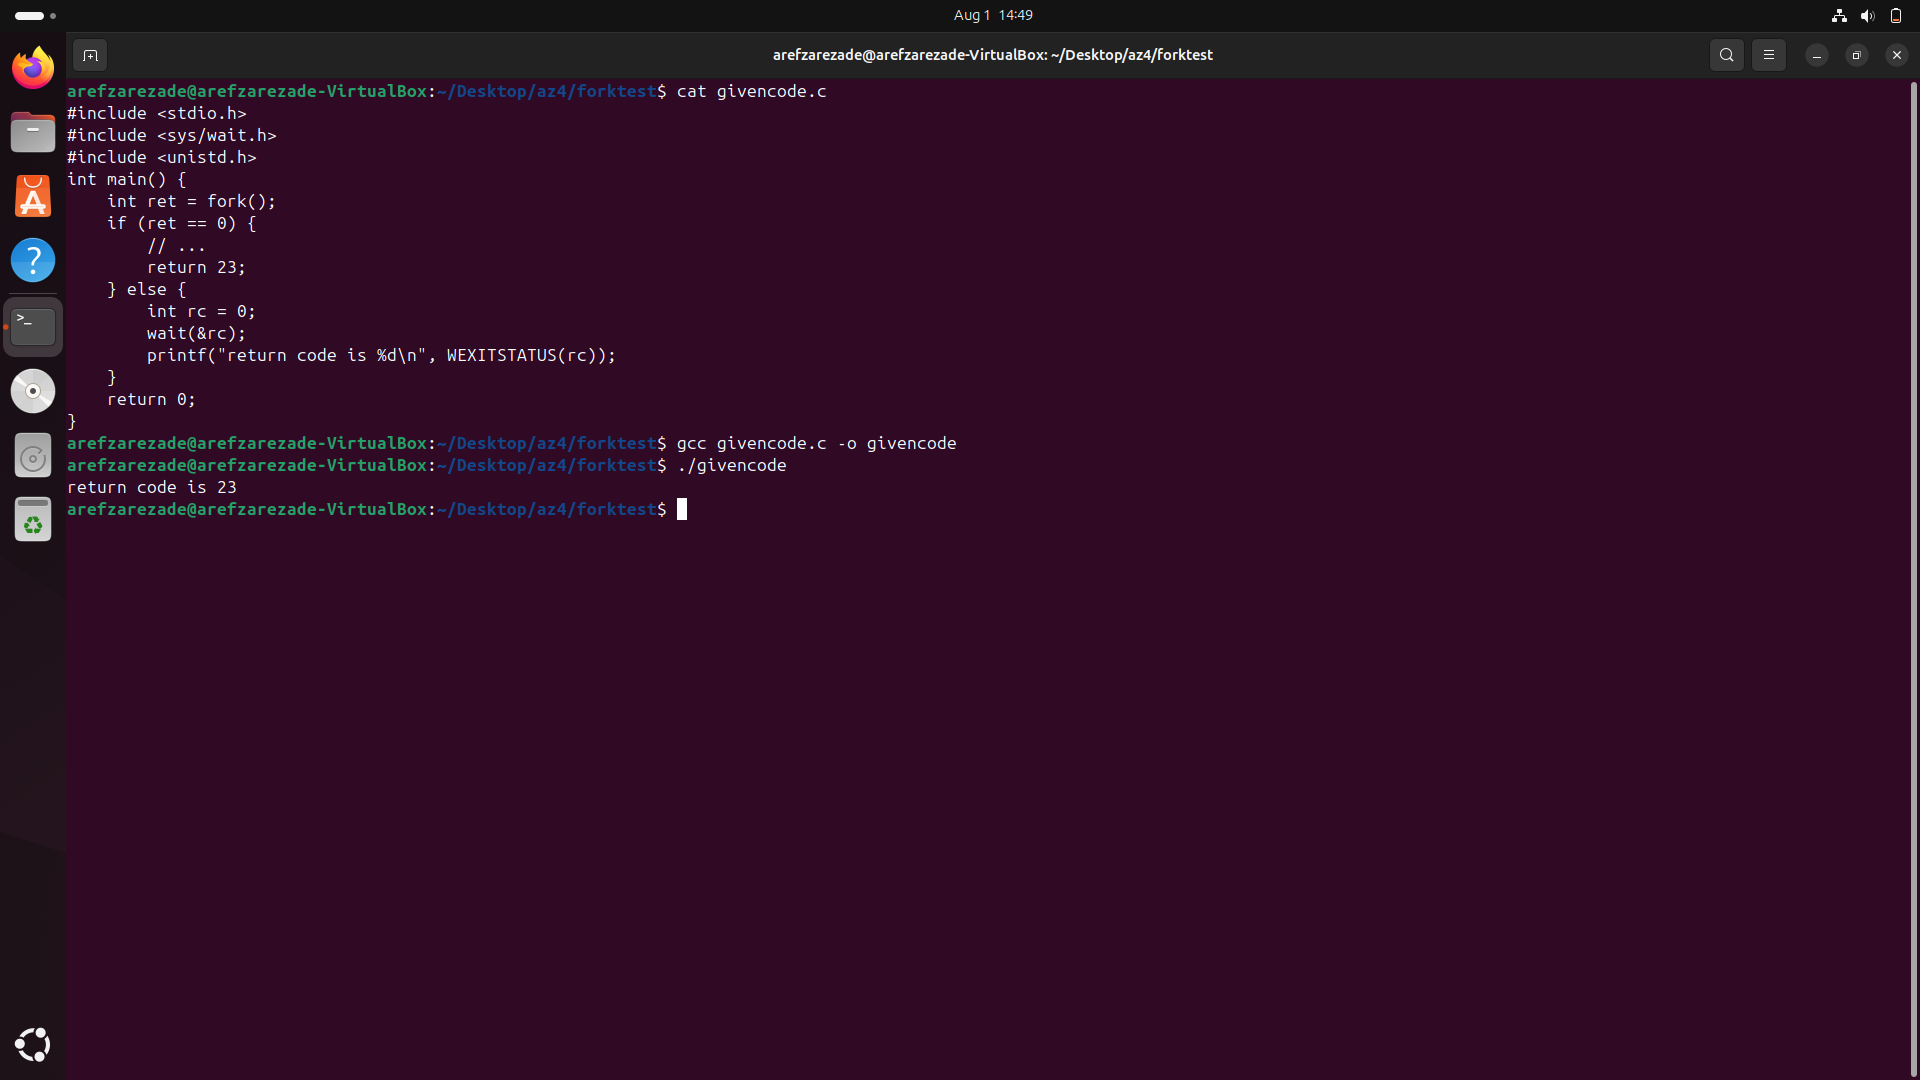
\includegraphics[width=0.8\textwidth]{report4-resources/5.png}
		\caption{ساخت پردازه‌ی جدید با \textenglish{fork()}}
            \label{im5}
	\end{figure}

        این کد ابتدا تابع
        \textenglish{fork()}
        را اجرا می‌کند. این تابع یک کپی از پردازه می‌سازد. خروجی تابع
        \textenglish{fork()}
        برای پردازه‌ی پدر،
        \textenglish{PID}
        فرزند است، و خروجی آن برای پردازه‌ی فرزند،
        \textenglish{0}
        است.

        سپس در 
        \textenglish{if}
        کد اجرا شده توسط پدر و فرزند جدا می‌شود. پردازه‌ی فرزند وارد
        \textenglish{if}
        شده و 
        \textenglish{23}
        را 
        \textenglish{return}
        می‌کند. پردازه‌ی پدر با دستور
        \textenglish{wait()}
        صبر می‌کند تا پردازه‌ی فرزند اجرایش تمام شده، سپس 
        \textenglish{status}
        مربوط به اتمام اجرای این پردازه‌ی فرزند در
        \textenglish{rc}
        ریخته می‌شود. همچنین با کمک ماکروی
        \textenglish{WEXITSTATUS()}،
        مقدار
        \textenglish{return value}
        پردازه‌ی فرزند را دریافت کرده و چاپ می‌کند.

        \item 
        برای اینکه مستقل بودن حافظه را نشان دهیم، به ابتدای کد بالا متغیر
        \textenglish{shared\_var}
        را با مقدار اولیه‌ی 
        \textenglish{1}
        اضافه می‌کنیم. در پردازه‌ی فرزند، مقدار آن را مساوی با 
        \textenglish{2}
        کرده و در پردازه‌ی پدر، پس از اتمام اجرای پردازه‌ی فرزند (با دستور
        \textenglish{wait()})
        مقدار این متغیر را چاپ می‌کنیم. همانطور که در شکل 
        \ref{im6}
        می‌توان مشاهده کرد، مقدار چاپ شده، همان مقدار 
        \textenglish{1}
        است. این نشان می‌دهد که  حافظه‌ی پردازه‌ی پدر و فرزند مستقل هستند و تغییرات در متغیرهای یکی، روی دیگری تاثیری ندارد.

        \begin{figure}[H]
		\centering
		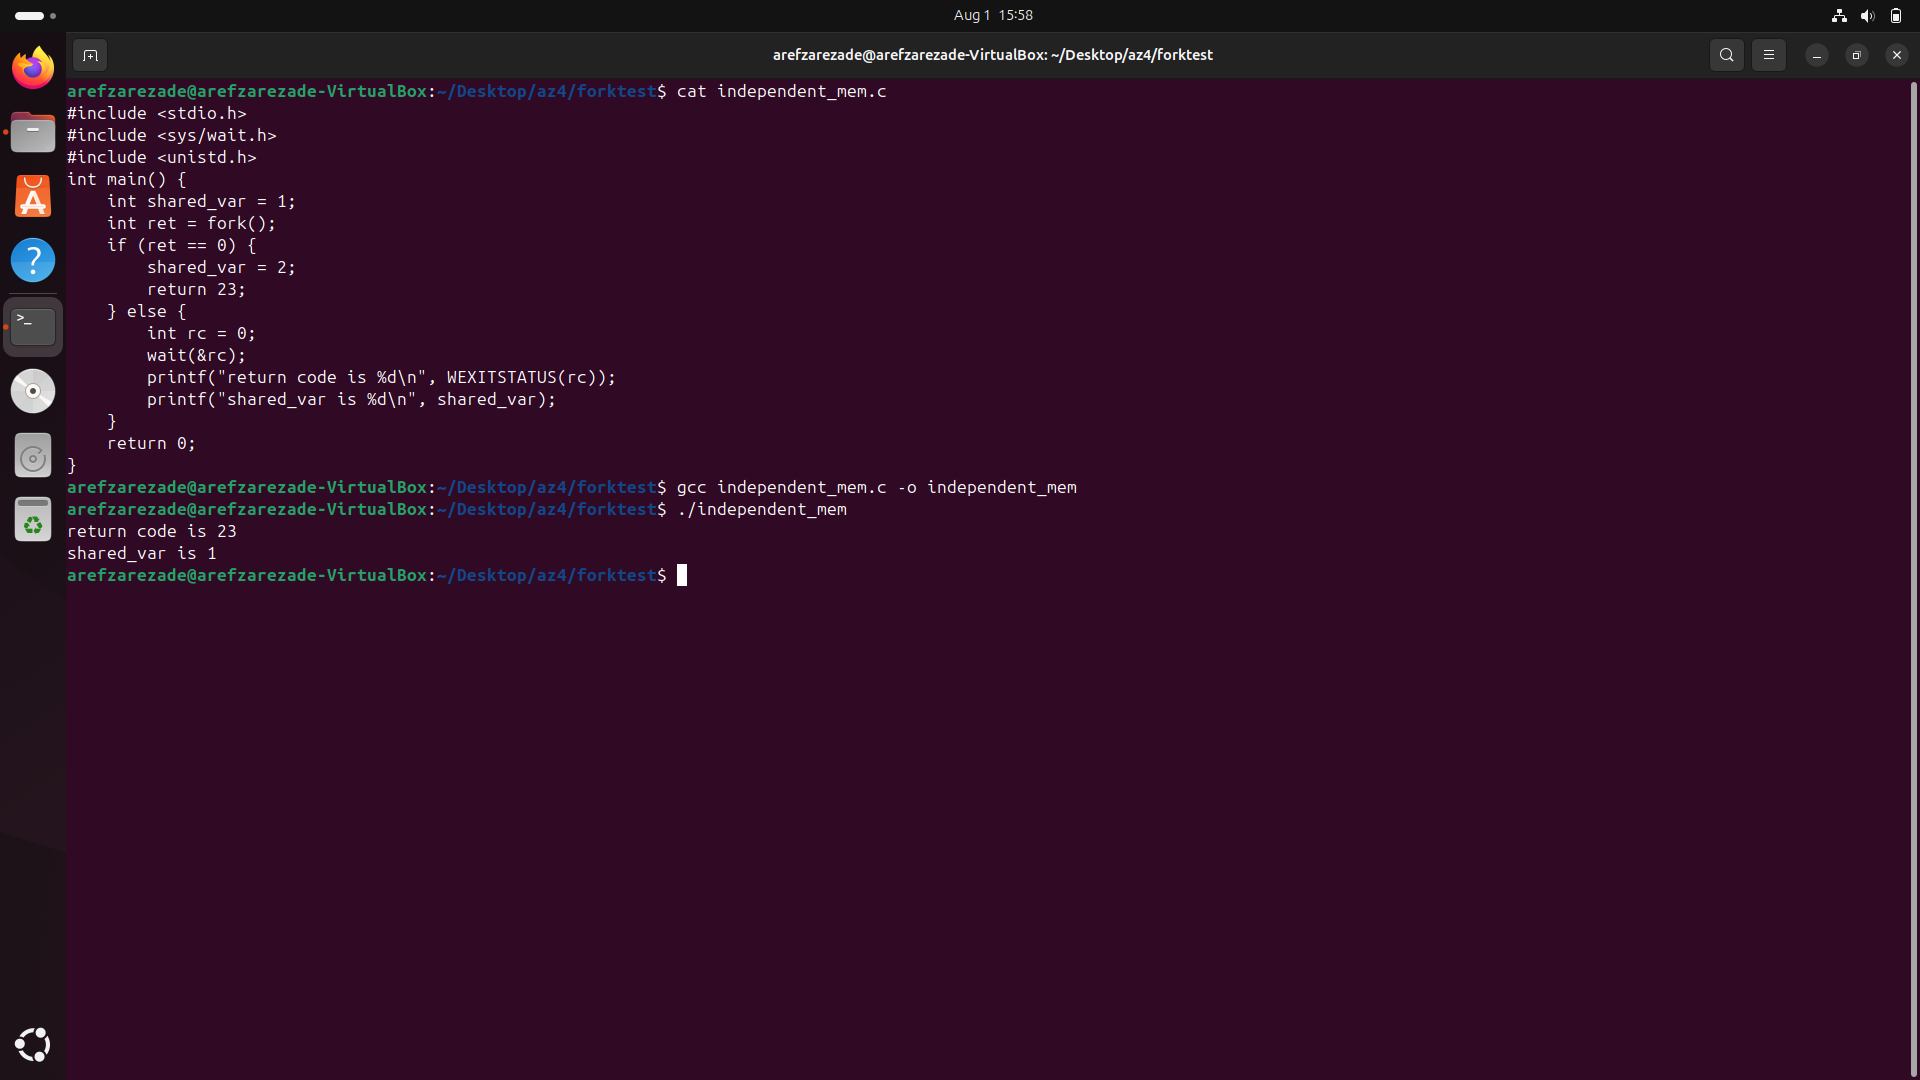
\includegraphics[width=0.8\textwidth]{report4-resources/6.png}
		\caption{بررسی مستقل بودن حافظه‌ی دو پردازه‌ی پدر و فرزند}
            \label{im6}
	\end{figure}

        \item 
        مانند کد بخش 2 عمل کرده، فقط در 
        \textenglish{if-else}،
        به جای کد آنها، دو عبارت 
        مختلف که شامل 
        \textenglish{PID}
        خودشان و پدرشان است را چاپ می‌کنیم. همچنین برای اینکه پردازه‌ی پدر، قبل از اجرای پردازه‌ی فرزند تمام نشود (و مقدار 
        \textenglish{ppid}
        چاپ شده مطابق انتظار باشد)، در انتهای کد مربوط به پدر، از دستور
        \textenglish{wait}
        استفاده کردیم.

        در شکل
        \ref{im7}
        می‌توانید کد و اجرای آن را ببنید.

        \begin{figure}[H]
		\centering
		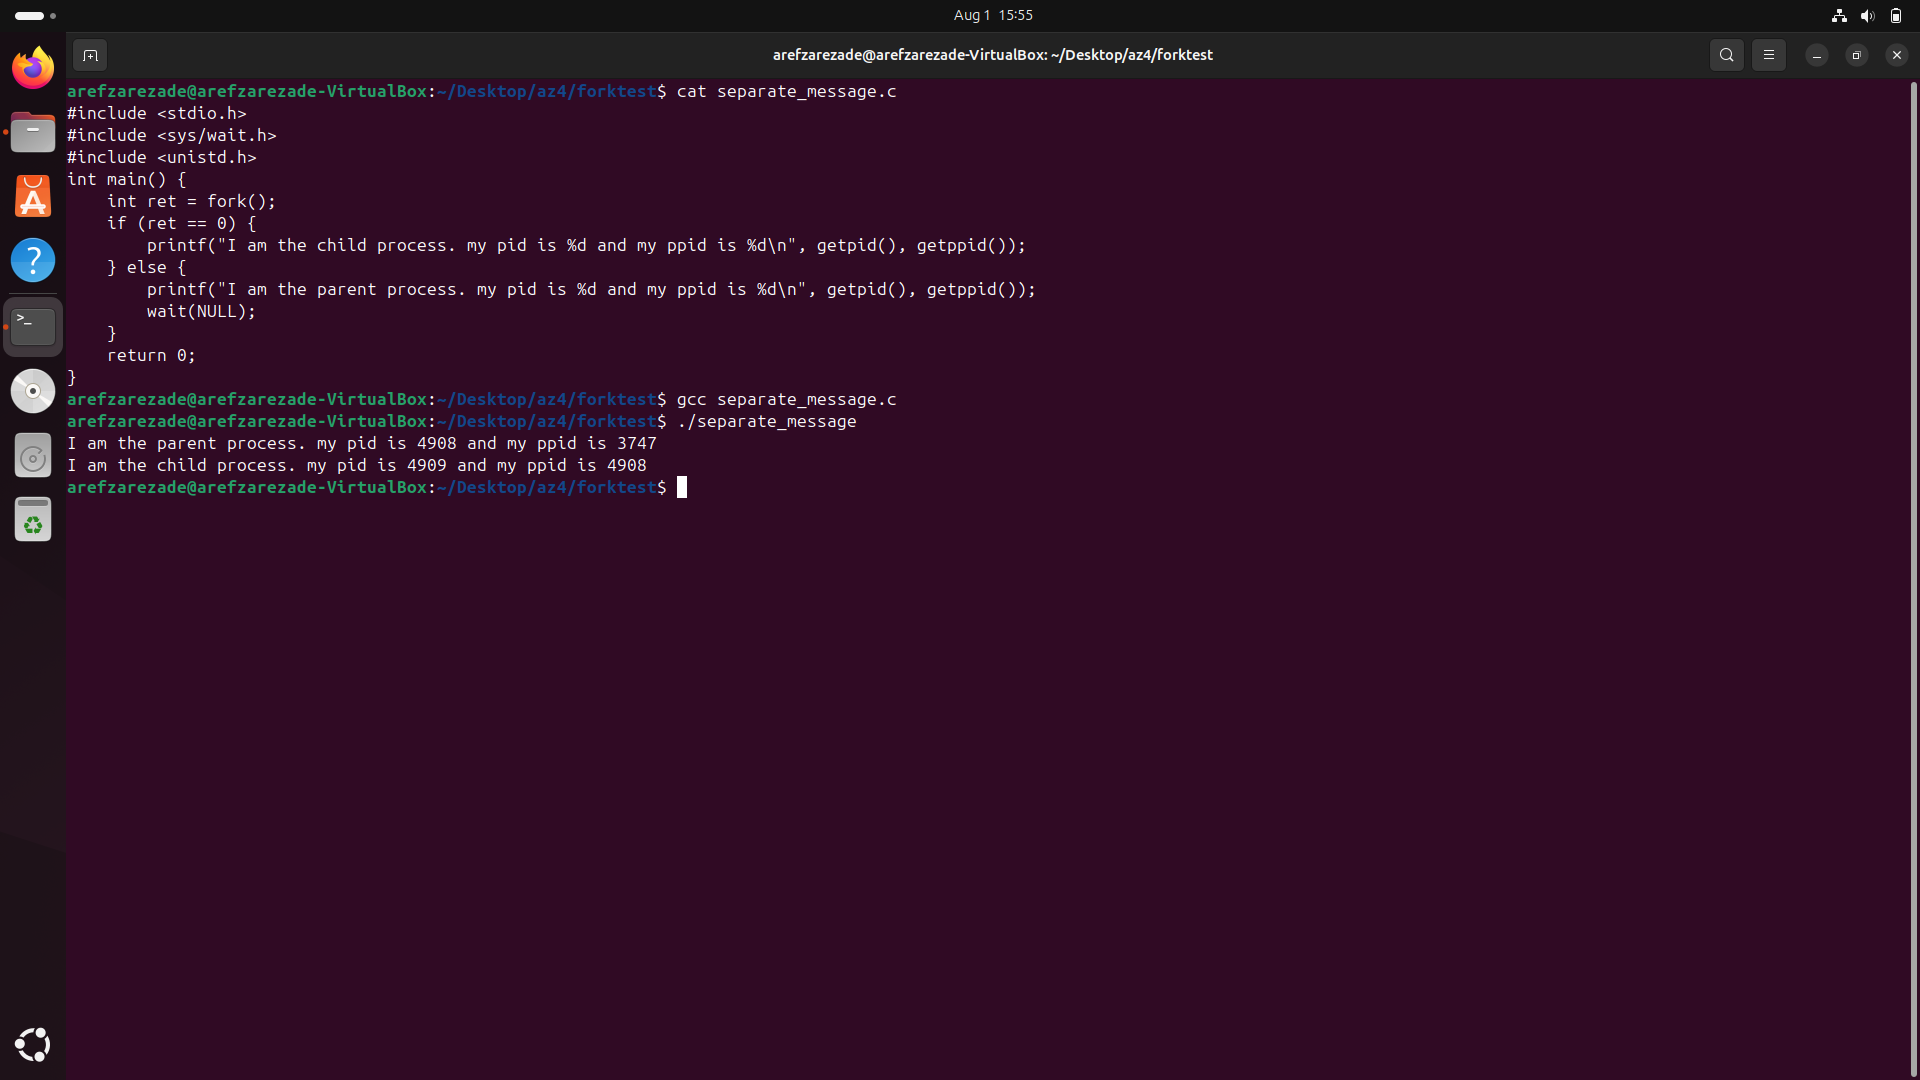
\includegraphics[width=0.8\textwidth]{report4-resources/7.png}
		\caption{چاپ عبارات مختلف توسط پردازه‌ی پدر و فرزند}
            \label{im7}
	\end{figure}

        \item 
        در شکل
        \ref{im8}
        می‌توان کد و همچنین خروجی آن را دید.

        \begin{figure}[H]
		\centering
		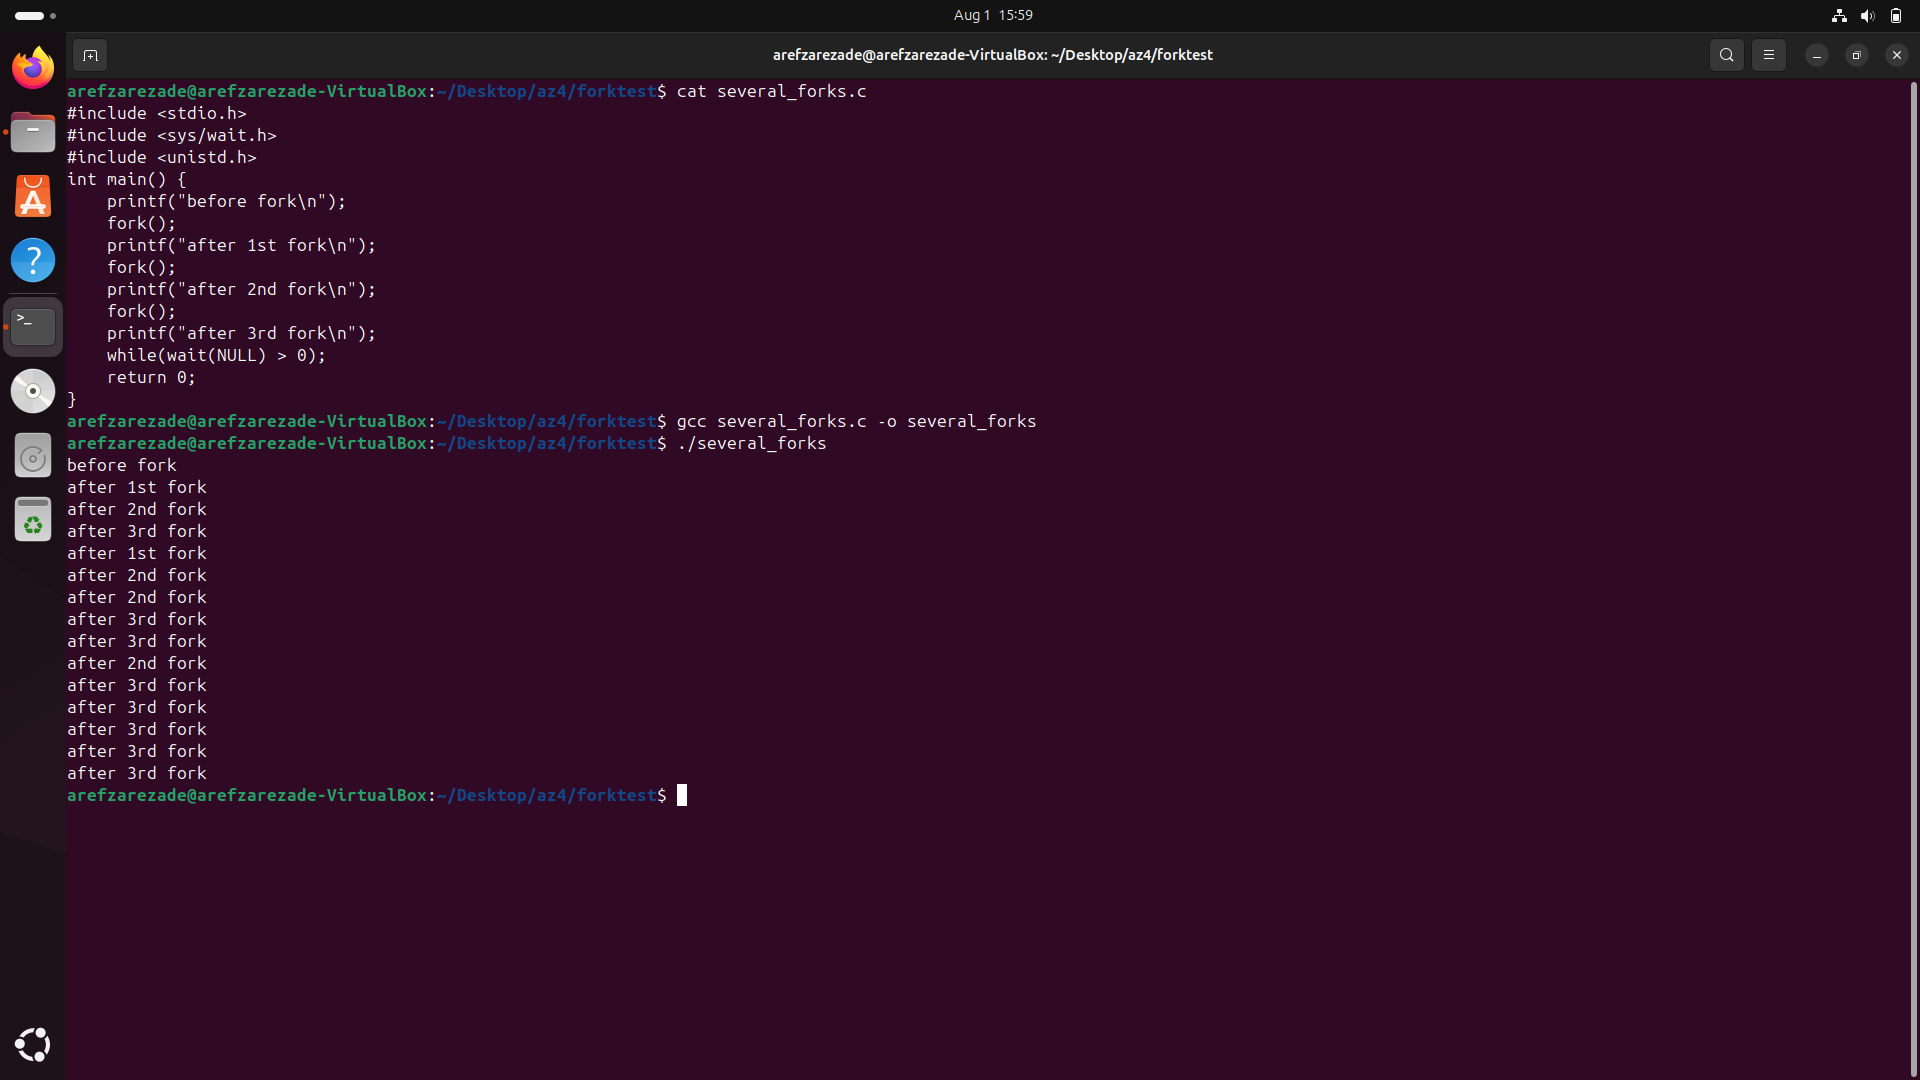
\includegraphics[width=0.8\textwidth]{report4-resources/8.png}
		\caption{وجود چند دستور \textenglish{fork} و چاپ عبارتی بینشان}
            \label{im8}
	\end{figure}

        همانطور که می‌توان مشاهده کرد، الگو و نظم خاصی در ترتیب اجرای پردازه‌های پدر یا فرزند وجود ندارد. هربار که با 
        \textenglish{fork}
        فرزند جدیدی ساخته می‌شود، معلوم نیست که پردازه‌ی فرزند ابتدا اجرا می‌شود، یا پردازه‌ی پدر، یا یکی از پردازه‌هایی که قبلا ساخته شده بودند.
        \end{enumerate}

        \subsection{اتمام کار پردازه‌ها}

        \begin{enumerate}
        \item 
        در شکل
        \ref{im9}
        می‌توانید کد خواسته شده را مشاهده کنید. این کد ابتدا با دستور
        \textenglish{fork}
        یک پردازه‌ی جدید می‌سازد. سپس با 
        \textenglish{if-else}
        شبیه به چیزی که در بخش‌های قبل دیدیم، کد اجرا شده‌ی پردازه‌ی پدر و فرزند را جدا می‌کند. در پردازه‌ی فرزند، عبارات 
        \textenglish{counting 1}
        تا 
        \textenglish{counting 100}
        چاپ شده، و در پردازه‌ی پدر با دستور
        \textenglish{wait(NULL)}
        (که صبر می‌کند تا یکی از پردازه‌های فرزند کارش تمام شود)،
        تا پابان اجرای پردازه‌ی فرزند کاری انجام نداده و سپس اتمام کار پردازه‌ی فرزند را اعلام می‌کند. چند خط انتهایی اجرای این برنامه را در شکل
        \ref{im10}
        می‌نوانید مشاهده کنید.

        \begin{figure}[H]
		\centering
		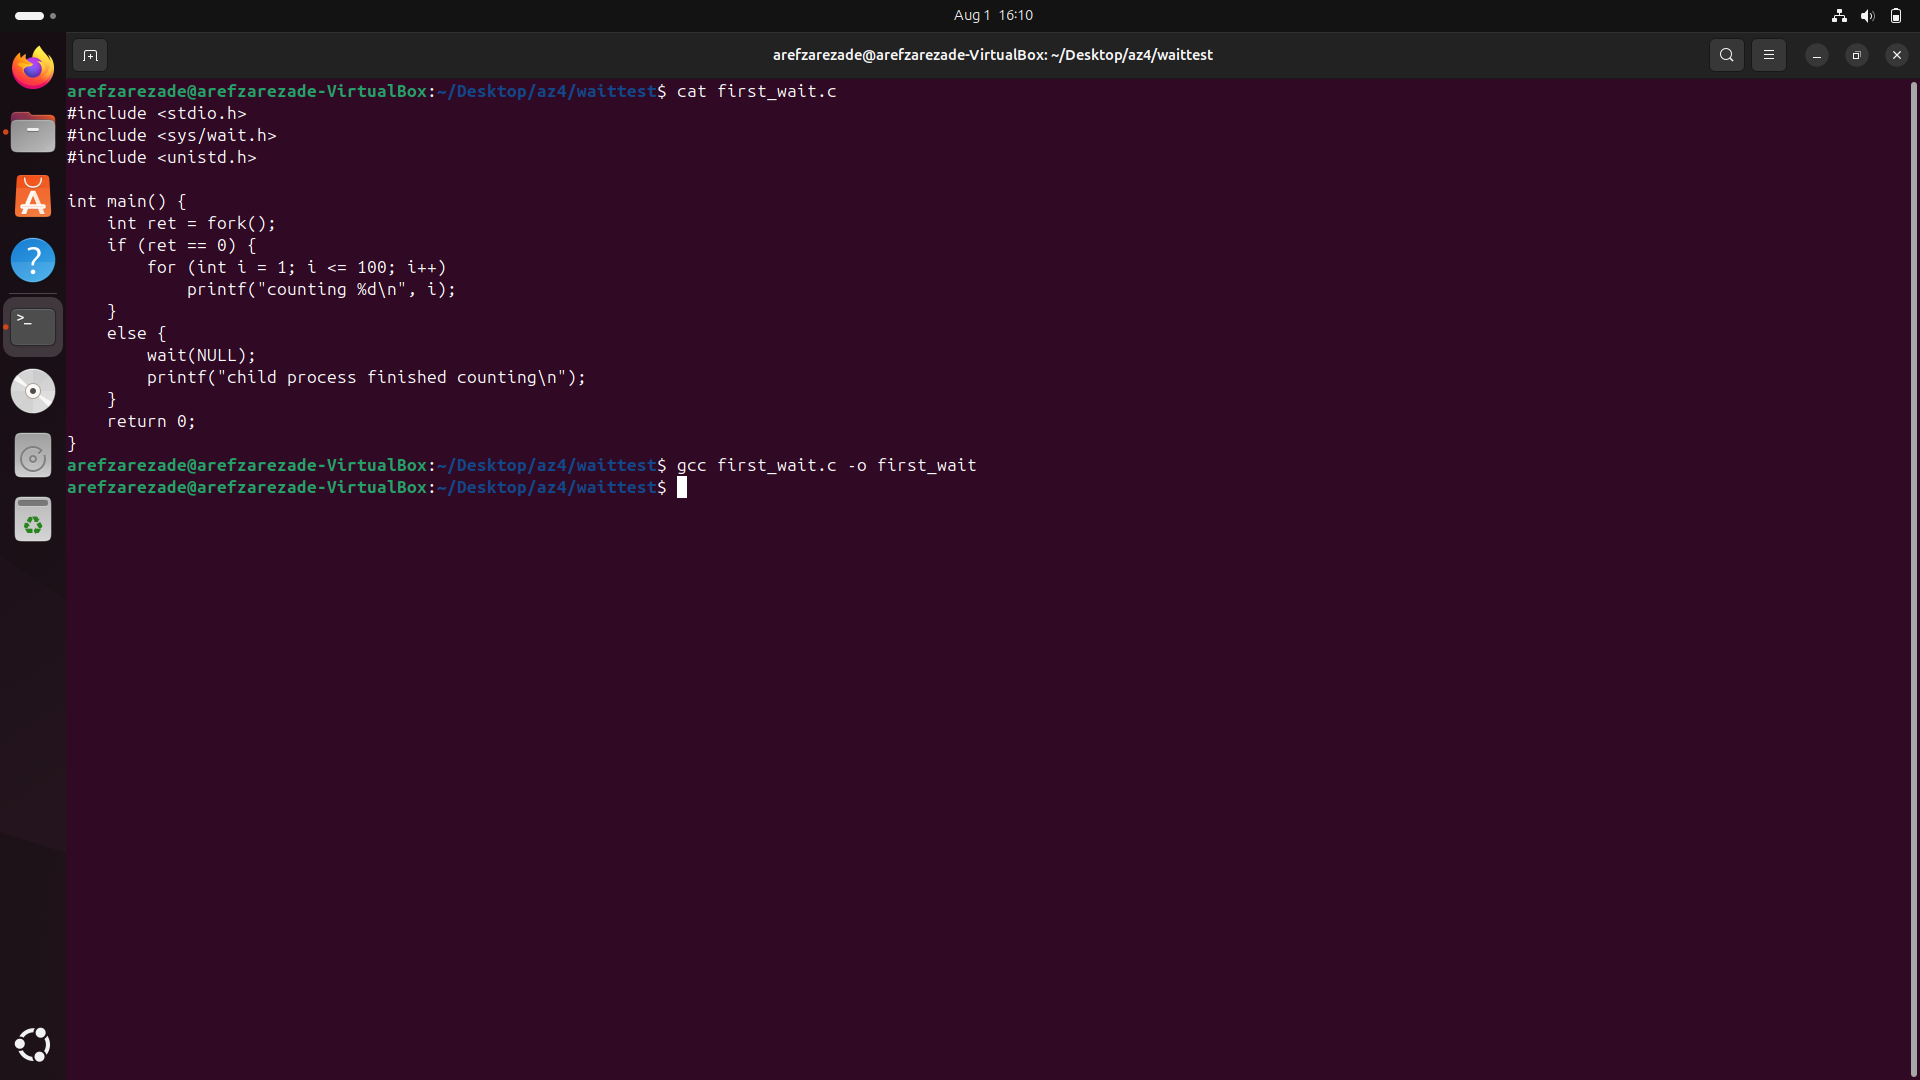
\includegraphics[width=0.8\textwidth]{report4-resources/9.png}
		\caption{کد صبر کردن برای اتمام اجرای پردازه‌ی فرزند}
            \label{im9}
	\end{figure}

        \begin{figure}[H]
		\centering
		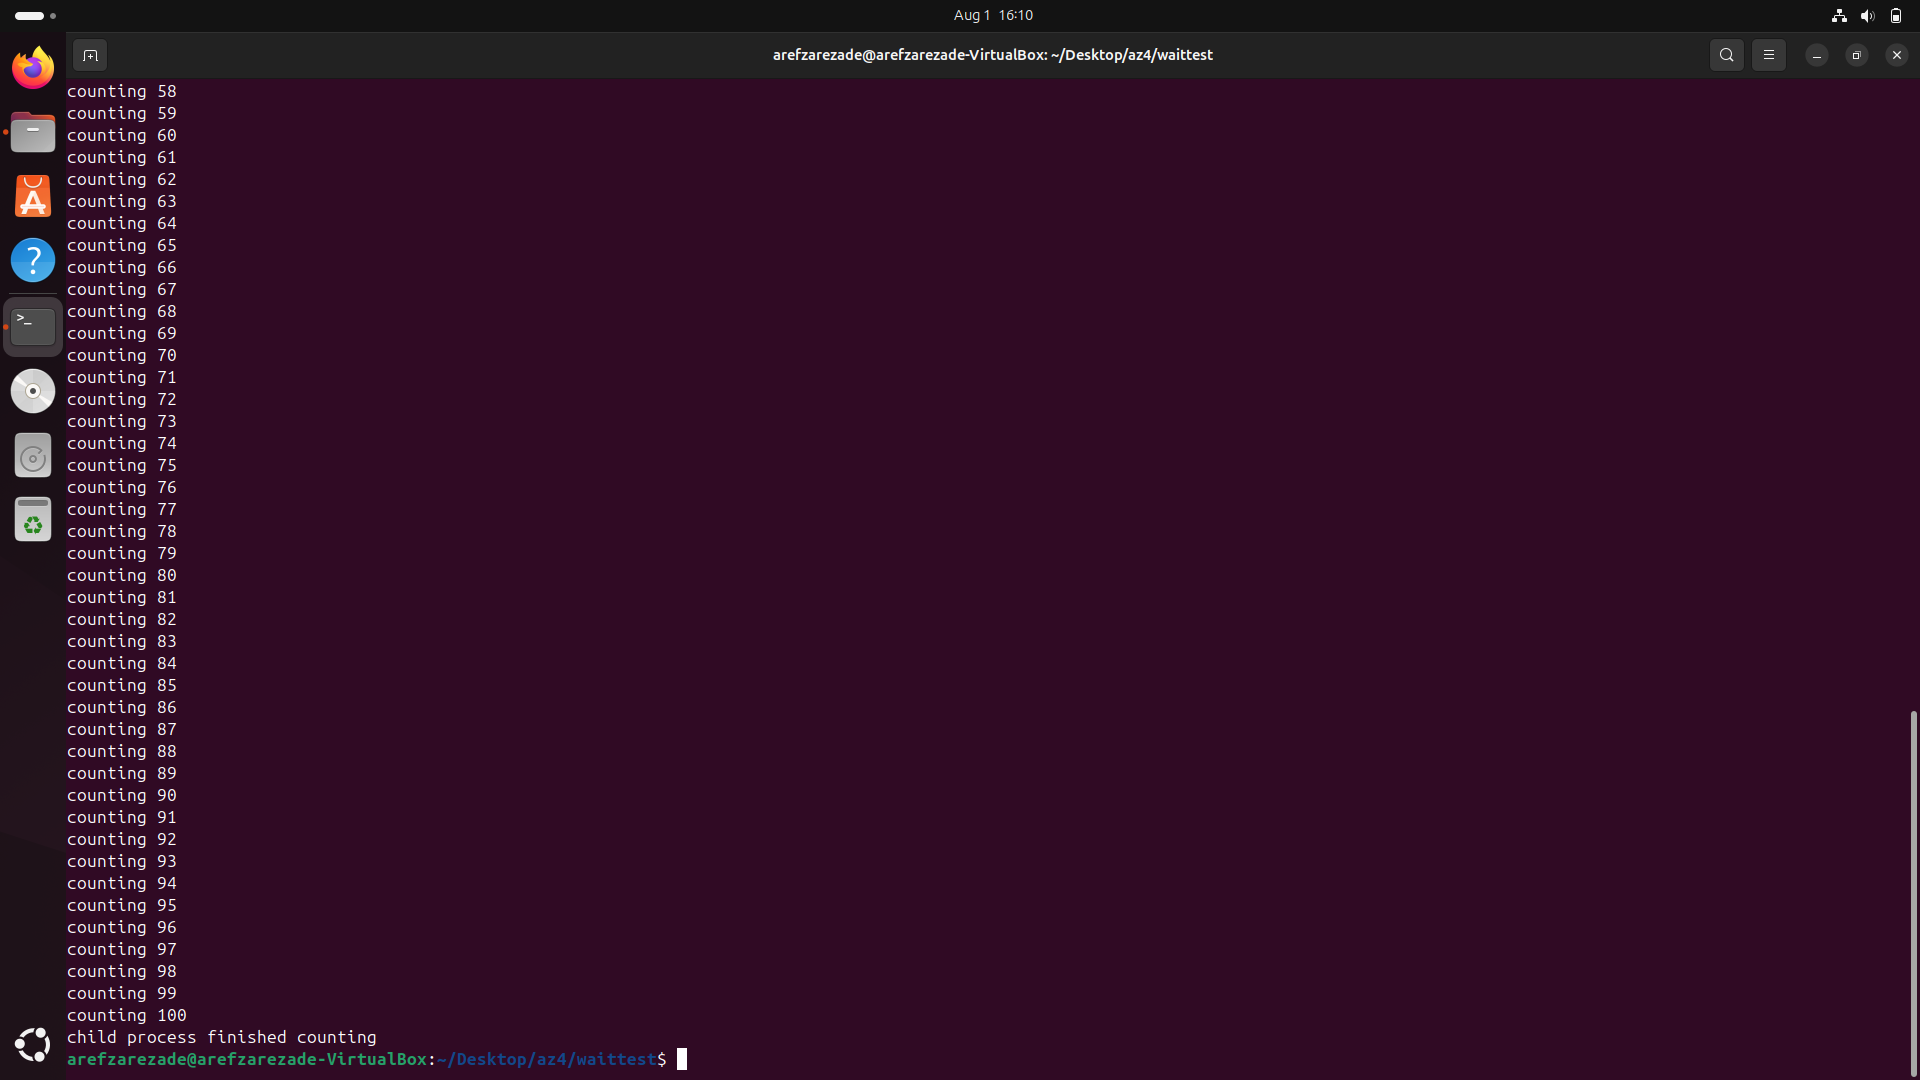
\includegraphics[width=0.8\textwidth]{report4-resources/10.png}
		\caption{اجرای کد مربوط به صبر کردن برای اتمام اجرای پردازه‌ی فرزند}
            \label{im10}
	\end{figure}

        \item 
        کد خواسته شده را در شکل
        \ref{im11}
        می‌توانید مشاهده کنید. در این کد، پردازه‌ی پدر به مدت 
        \textenglish{1}
        ثانیه صبر کرده و سپس اجرایش تمام می‌شود. پردازه‌ی فرزند ابتدا 
        \textenglish{PID}
        خودش و پدرش را چاپ می‌کند، سپس 
        \textenglish{2}
        ثانیه صبر می‌کند. پس از این دو ثانیه، پردازه‌ی پدر به طور قطع کارش تمام می‌شود. سپس
        \textenglish{PID}
        خودش و پدر جدیدش را چاپ می‌کند. 

        همانطور که می‌توان مشاهده کرد، پردازه‌ی پدر جدید، پردازه‌ی
        \textenglish{systemd}
        که همان 
        \textenglish{init}
        است می‌باشد. البته در این مورد، 
        \textenglish{PID}
        آن 
        \textenglish{1}
        نیست. دلیل آن این است که این یک نمونه از پردازه‌ی
        \textenglish{systemd}
        که مختص به کاربر است می‌باشد، و نه 
        \textenglish{systemd}
        مربوط به سیستم (که در ابتدای بالا آمدن سیستم اجرا می‌شود).

        \begin{figure}[H]
		\centering
		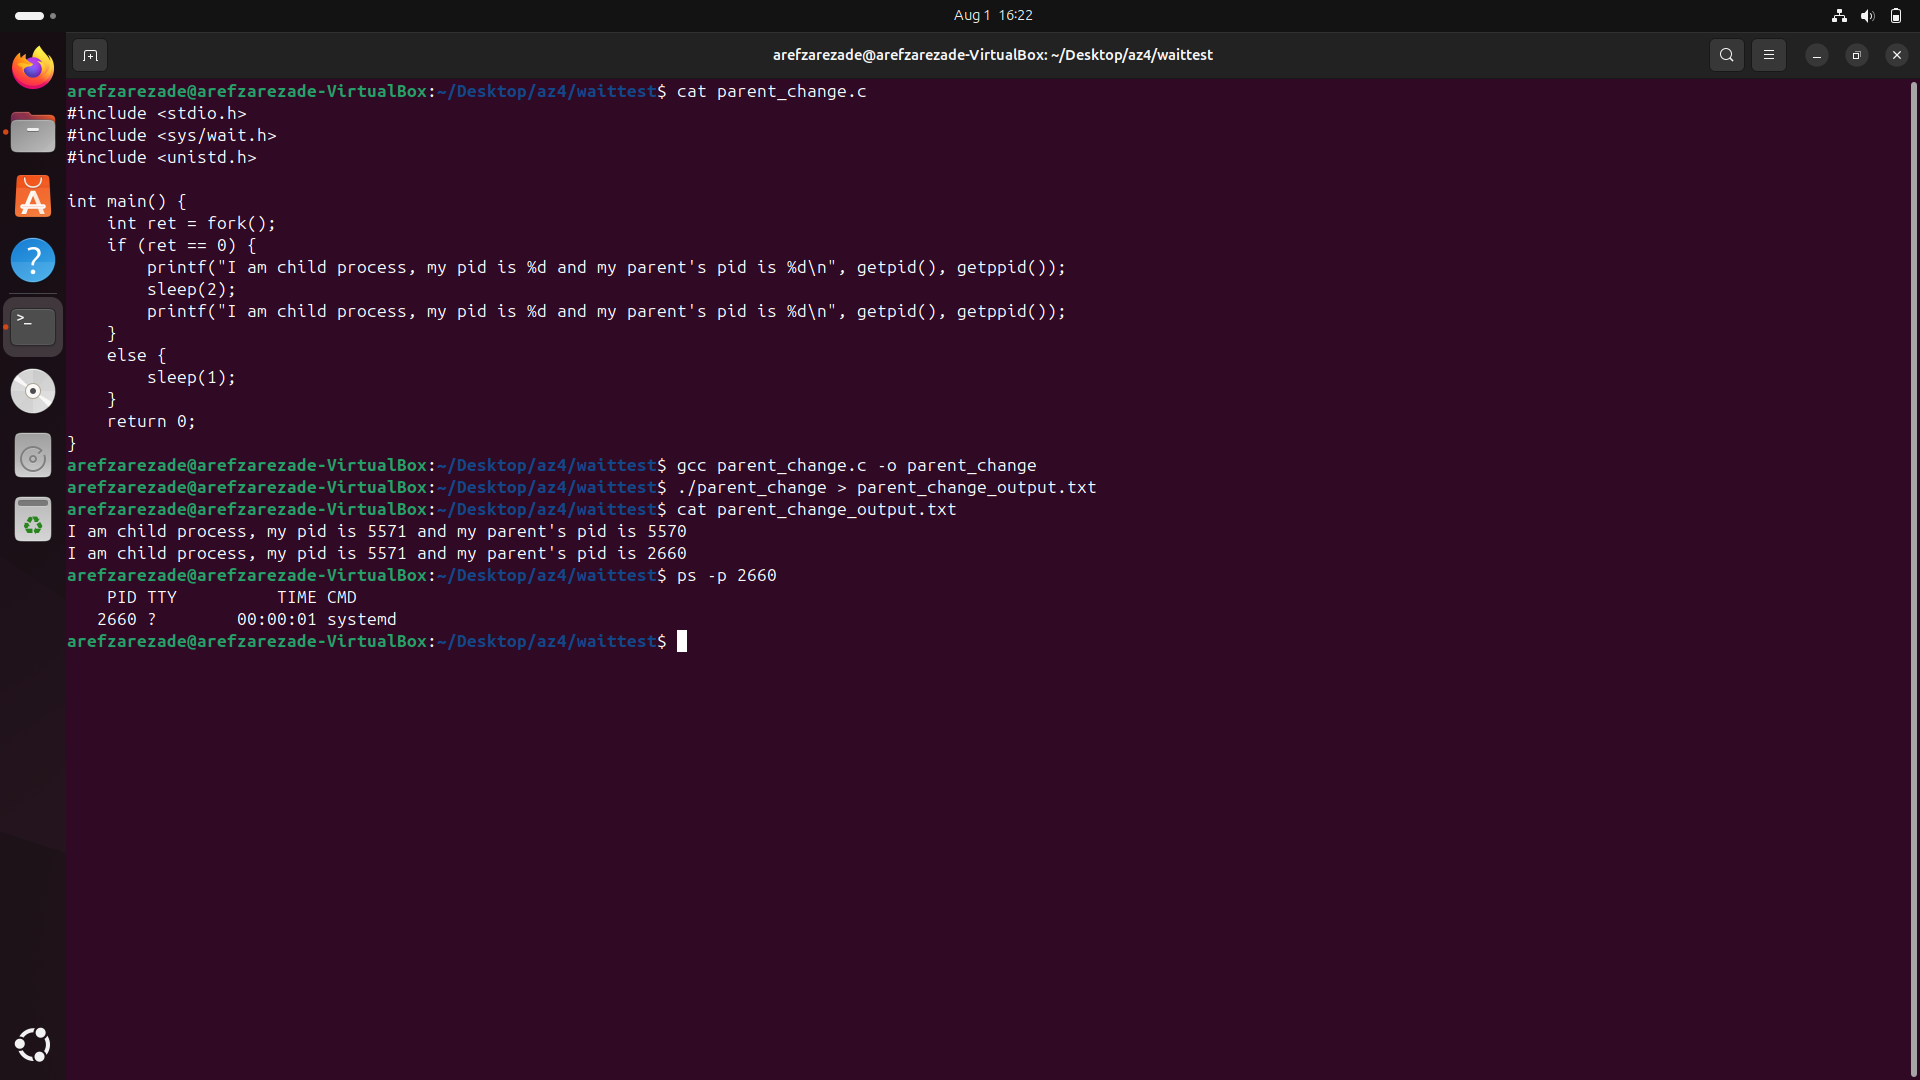
\includegraphics[width=0.8\textwidth]{report4-resources/11.png}
		\caption{گرفتن پدر جدید توسط پردازه‌ی فرزند، پس از اتمام اجرای پدر اصلی}
            \label{im11}
	\end{figure}
        \end{enumerate}

        \subsection{اجرای فایل}
        \begin{enumerate}
        \item 
        تفاوت اصلی این دستورات در نحوه‌ی گرفتن آرگومان‌های ورودی، و تعامل با برنامه‌های موجود در
        \textenglish{PATH}
        است. این تفاوت‌ها را در جدول
        \ref{tab1}
        ‌می‌توانید مشاهده کنید.

        \begin{table}[h!]
            \centering
            \begin{tabular}{|c|c|c|c|}
            \hline
            نام تابع & فرمت گرفتن آرگومان‌ها & آیا \textenglish{PATH} را جستجو می‌کند؟ \\
            \hline
            \texttt{execl}   & تمام آرگومان‌ها در ورودی تابع & خیر \\
            \texttt{execv}   & آرایه‌ای از آرگومان‌ها & خیر \\
            \texttt{execlp}  & تمام آرگومان‌ها در ورودی تابع & بله \\
            \texttt{execvp}  & آرایه‌ای از آرگومان‌ها & بله  \\
            \hline
            \end{tabular}
            \caption{مقایسه‌ی دستورات \texttt{exec}}
            \label{tab1}
        \end{table}

        \item 
        کد این برنامه و نمونه‌ی اجرا شدن آن را در شکل 
        \ref{im12}
        می‌توانید مشاهده کنید. در این برنامه، ابتدا با دستور 
        \textenglish{fork}
        یک پردازه‌ی جدید ساخته شده، سپس پردازه‌ی فرزند با دستور
        \textenglish{execlp}،
        دستور خواسته شده را انجام می‌دهد. البته طبق راهنمایی، دو بار باید 
        \textenglish{ls}
        را در آرگومان‌های تابع
        \textenglish{execlp}
        بیاوریم. دلیل آن این است که اولین
        \textenglish{ls}
        نشان می‌دهد کدام دستور/برنامه باید اجرا شود، و دومین
        \textenglish{ls}
        مربوط به آرگومان اول دستور اجرا شده که همان
        \textenglish{ls g h}
        است می‌باشد.

        \begin{figure}[H]
		\centering
		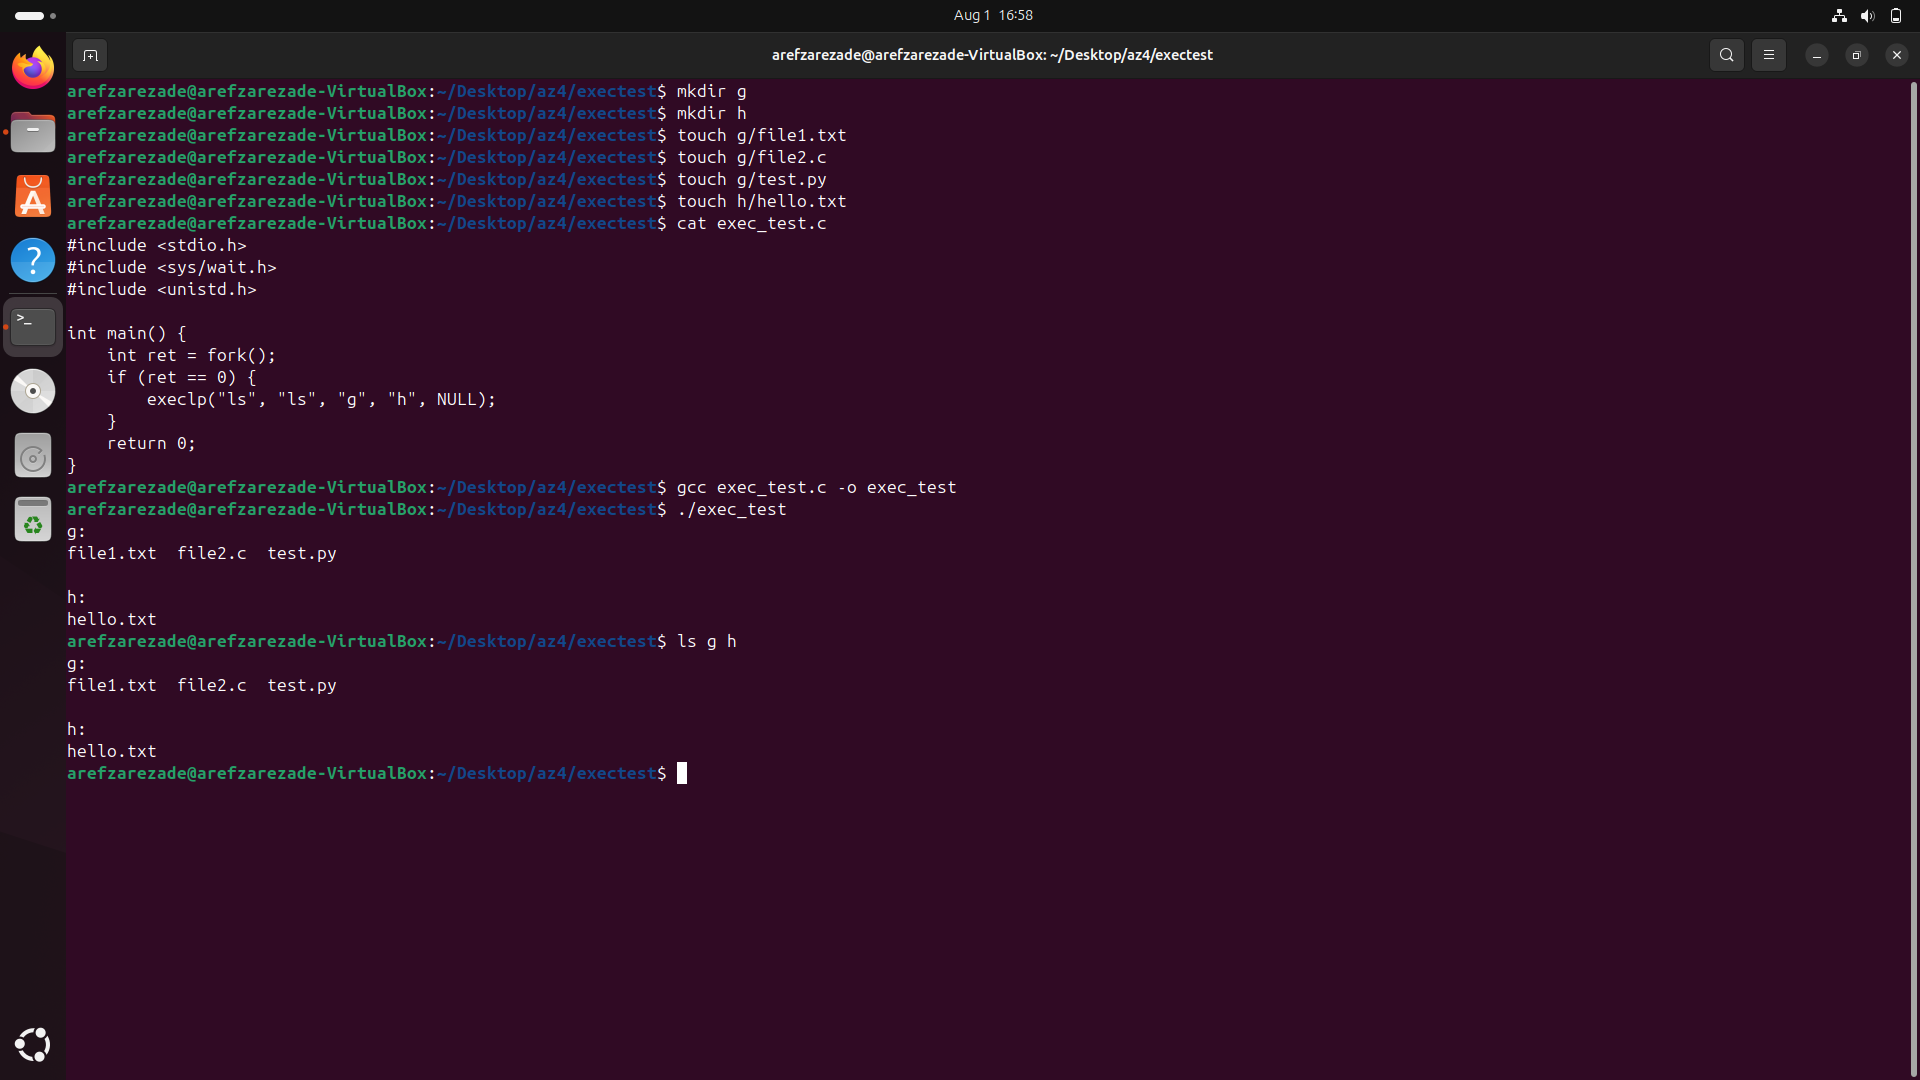
\includegraphics[width=0.8\textwidth]{report4-resources/12.png}
		\caption{اجرای برنامه توسط پردازه‌ی فرزند با کمک \textenglish{execlp}}
            \label{im12}
	\end{figure}
        \end{enumerate}

        \section{فعالیت‌ها}

        \begin{itemize}
        \item 
        گروه‌های پردازه‌ای برای گروه‌بندی پردازه‌های مشابه و سادگی در انجام بعضی کارها وجود دارند. از کاربردهای آن می‌توان به این موضوع که 
        \textenglish{signal broadcasting}
        وجود دارد اشاره کرد. به این صورت که با اجرای یک دستور، می‌توان سیگنالی را به همه‌ی پردازه‌های آن گروه فرستاد اشاره کرد\cite{man7-credentials}. گروه‌بندی پردازه‌ها در جاهایی مانند 
        \textenglish{pipeline}
        کردن دستورات نیز کاربرد دارد. 

        دستورات
        \textenglish{setpgid}
        و 
        \textenglish{getpgrp}
        به ترتیب برای گروه‌بندی پردازه (اضافه کردن یک پردازه به یک گروه) و گرفتن 
        \textenglish{group ID}
        پردازه به کار می‌روند
        \cite{man7-setpgid}.

        نحوه‌ی اجرا کردن
        \textenglish{setpgid}
        به این صورت است:

        \begin{english}
            setpgid(pid, pgid)
        \end{english}

        آرگومان اول، 
        \textenglish{PID}
        پردازه‌ای است که می‌خواهیم آن را گروه بندی کنیم. اگر
        \textenglish{0}
        باشد، به معنای پردازه‌ای که آن را صدا کرده است می‌باشد.

        آرگومان دوم،
        \textenglish{PGID}
        یا
        \textenglish{group ID}
        مربوط به گروهی که می‌خواهیم پردازه را در آن قرار دهیم است. اگر 
        \textenglish{0}
        باشد، به معنای این است که
        \textenglish{PGID}
        را مساوی با 
        \textenglish{PID}
        قرار دهیم.


        \item 
        درخت آن به صورت زیر است. در درخت زیر، هر راس میانی را یک
        \textenglish{fork}
        در نظر گرفته، و فرض کرده‌ایم پردازه‌ی پدر راس سمت چپ بعد از
        \textenglish{fork}
        است، و پردازه‌ی فرزند سمت راست. همچنین هر برگ، پردازه‌ای است که به عبارت چاپ شده رسیده است. همچنین خروجی این کد را در شکل
        \ref{im13}
        می‌توانید مشاهده کنید.

        
        \begin{center}
            \begin{tikzpicture}[scale=0.2]
            \tikzstyle{every node}+=[inner sep=0pt]
            \draw [black] (37,-14.4) circle (3);
            \draw (37,-14.4) node {$fork1$};
            \draw [black] (27,-26.9) circle (3);
            \draw (27,-26.9) node {$fork2$};
            \draw [black] (46.3,-26.9) circle (3);
            \draw (46.3,-26.9) node {$fork2$};
            \draw [black] (13.2,-38.6) circle (3);
            \draw [black] (28.2,-38.6) circle (3);
            \draw [black] (44.1,-37.8) circle (3);
            \draw [black] (57.1,-37.8) circle (3);
            \draw [black] (35.13,-16.74) -- (28.87,-24.56);
            \fill [black] (28.87,-24.56) -- (29.76,-24.25) -- (28.98,-23.62);
            \draw (31.44,-19.23) node [left] {$parent$};
            \draw [black] (38.79,-16.81) -- (44.51,-24.49);
            \fill [black] (44.51,-24.49) -- (44.43,-23.55) -- (43.63,-24.15);
            \draw (42.23,-19.26) node [right] {$child$};
            \draw [black] (24.71,-28.84) -- (15.49,-36.66);
            \fill [black] (15.49,-36.66) -- (16.42,-36.52) -- (15.78,-35.76);
            \draw (17.09,-32.26) node [above] {$parent$};
            \draw [black] (27.31,-29.88) -- (27.89,-35.62);
            \fill [black] (27.89,-35.62) -- (28.31,-34.77) -- (27.31,-34.87);
            \draw (28.24,-32.66) node [right] {$child$};
            \draw [black] (45.71,-29.84) -- (44.69,-34.86);
            \fill [black] (44.69,-34.86) -- (45.34,-34.17) -- (44.36,-33.98);
            \draw (44.46,-32.03) node [left] {$parent$};
            \draw [black] (48.41,-29.03) -- (54.99,-35.67);
            \fill [black] (54.99,-35.67) -- (54.78,-34.75) -- (54.07,-35.45);
            \draw (52.22,-30.87) node [right] {$child$};
            \end{tikzpicture}
        \end{center}

        \begin{figure}[H]
		\centering
		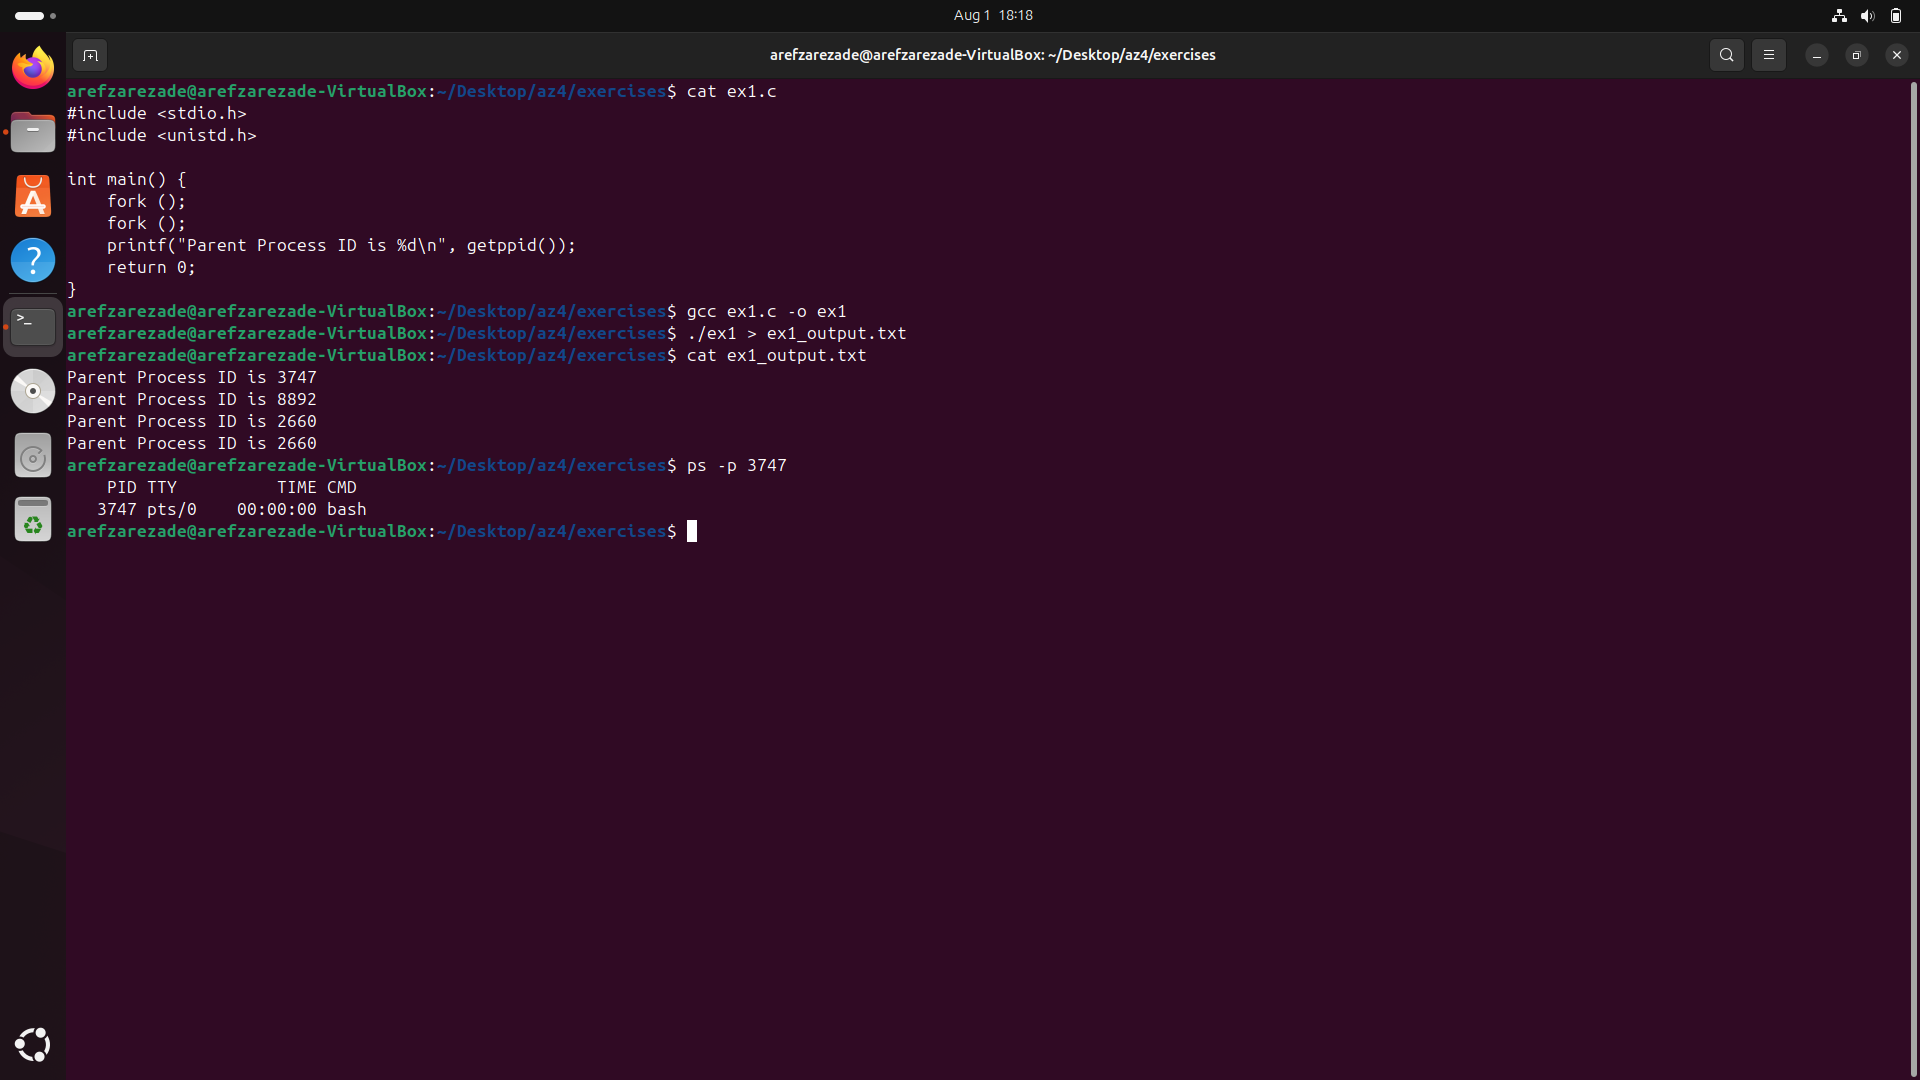
\includegraphics[width=0.8\textwidth]{report4-resources/13.png}
		\caption{خروجی برنامه‌ی دارای دو \textenglish{fork}}
            \label{im13}
	\end{figure}
        
        \item 
        این برنامه را با یک تغییر کوچک اجرا کردیم، و آن تغییر کوچک
        \textenglish{flush}
        کردن 
        \textenglish{stdout}
        پس از هر عبارت
        \textenglish{printf}
        است. دلیل این کار این است که بتوان خروجی کد را در فایل ریخت، و خروجی آن مانند خروجی هنگام اجرای آن در ترمینال باشد. سپس مطابق شکل
        \ref{im14}،
        سه بار این کد را اجرا کرده و خروجی‌ها را کنار هم می‌گذاریم.

        \begin{figure}[H]
		\centering
		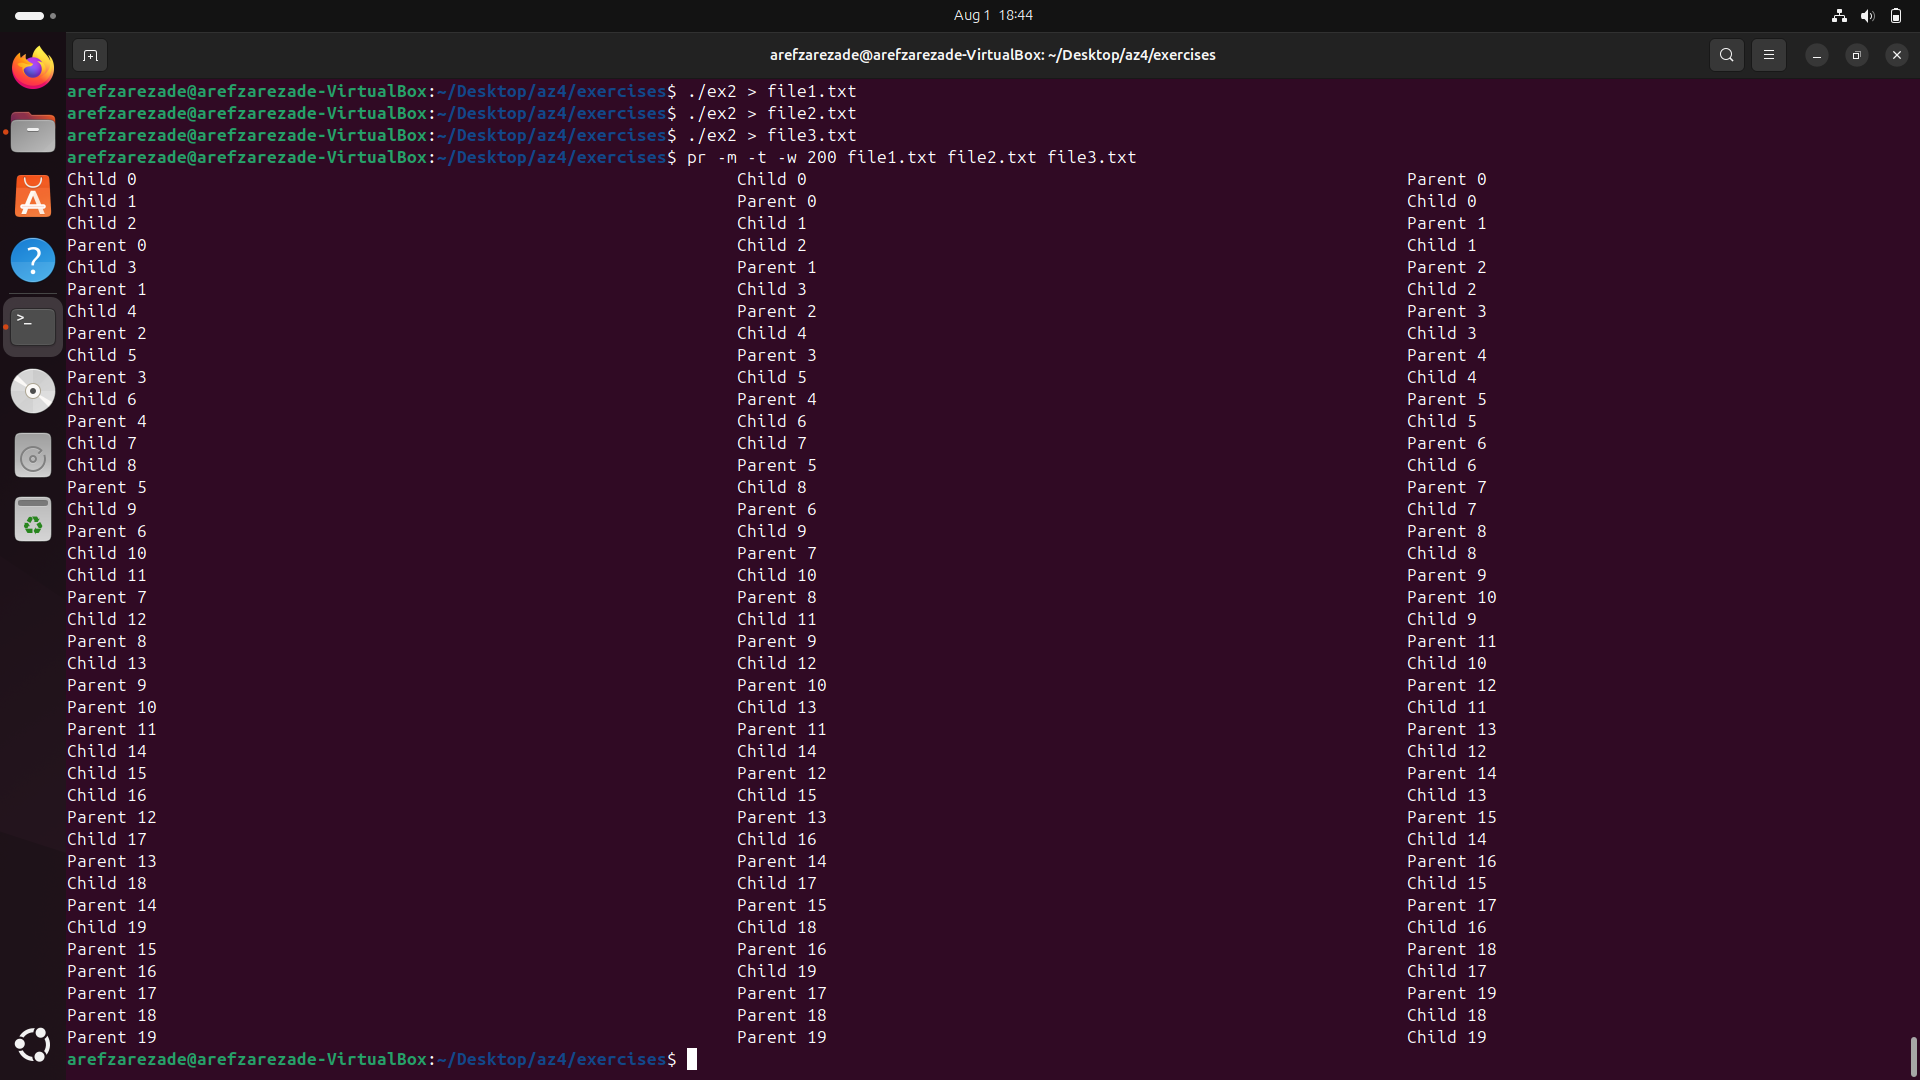
\includegraphics[width=0.8\textwidth]{report4-resources/14.png}
		\caption{چند بار اجرای کد طولانی دارای \textenglish{fork}}
            \label{im14}
	\end{figure}

        همانطور که از بی‌نظمی ترتیب عبارات چاپ شده می‌توان دید، ترتیب اجرای پردازه‌های پدر و فرزند الگوی خاصی ندارد و ترتیب اجرای آنها توسط سیستم عامل به ظاهر تصادفی به نظر می‌رسد.

        \item 
        پردازه‌ی
        \textenglish{zombie}
        پردازه‌ای است که اجرای آن تمام شده، اما هنوز در 
        \textenglish{process table}
        سیستم عامل وجود دارد
        \cite{wikipedia-zombie-process}.

        دلیل حذف نشدن آن این است که پردازه‌ی پدر با دستوراتی مانند 
        \textenglish{wait}
        وضعیت خروجی آن را دریافت نکرده است. از طرفی، سیستم عامل نمی‌تواند خودش آن را از جدول پردازه‌ها حذف کند، زیرا ممکن است در آینده، پردازه‌ی پدر با دستور
        \textenglish{wait}
        یا دستورات مشابه، بخواهد وضعیت خروجی آن پردازه را بررسی کند.

        
        \end{itemize}

        
        
	
	% ==============================
	% References
	% ==============================
	\newpage
	\begin{LTR}
		\begin{english}
\printbibliography[title={مراجع}]
\end{english}
	\end{LTR}

	
\end{document}

